\documentclass[10pt]{article}
%%%%%%%%%%%%%%%%%%%%%%%  ПАКЕТЫ  %%%%%%%%%%%%%%%%%%%%%%%%%%%%%%%%%%%%%%%%%%%%%%
\usepackage{cmap}                               % Чтобы в PDF работал человеческий поиск
\usepackage[X2,T2A]{fontenc}                    % T2A = русская кодировка. X2 = яти
\usepackage[utf8]{inputenc}                     % Ввод в универсальной кодировке
\usepackage{setspace,soulutf8}      		        % Чтобы можно было менять межстрочный и межбуквенный интервалы
\usepackage{amsmath,amsfonts,amssymb,amsthm}    % Символы для математики
\usepackage{mathrsfs}                           % Символы для математики
\usepackage{dsfont}                             % Шрифт для знака индикатора
\usepackage[subfigure]{tocloft}  % Многоточие в оглавлении
\usepackage{array,multicol,multirow,bigstrut}   % Чтобы можно было делать в таблице колонки фиксированной ширины, слитные ячейки, вставлять strut'ы.
\usepackage{indentfirst}                        % Абзацный отступ везде
\usepackage[british,russian]{babel}                     % Русские переносы, тире, типографика, самодержавие, духовность!
\usepackage[perpage]{footmisc}                  % Сброс счётчика сносок на каждой странице
\usepackage[pdftex,unicode,bookmarks=true,bookmarksopen=true,colorlinks=true,linkcolor=blue,urlcolor=blue,citecolor=blue]{hyperref} % Синие ссылки в PDF
\usepackage{microtype}                          % Свешивающаяся пунктуация и подгонка белого пространства по правилу \pm 2 процента
\usepackage{textcomp}                           % Чтобы в формулах можно было русские буквы писать через \text{}
\usepackage[paper=a4paper,top=12.7mm, bottom=5.7mm,left=5.7mm,right=12.7mm,bindingoffset=6.6mm,includefoot]{geometry} % Достаточно экономные размеры листа и поля для нумерации страниц внизу (для колонтитулов в стиле лекций по матану, нужно includefoot заменить на includehead и не только
\usepackage{xcolor}                             % Чтобы можно было цветные объекты вставлять
\usepackage[pdftex]{graphicx}                   % Чтобы вставились изображения
\usepackage{float,longtable}                    % Поддержка плавающих таблиц и рисунков
\usepackage[margin=0pt,font=small,labelfont=bf,labelsep=period]{caption} % Подписи таблиц и рисунком мелкие, жирные, с принятым в русской типографике разделителем.
\usepackage{rotating}                   % Создание своих акцентов, поворот объекта.
\usepackage{datetime}                           % Отображение времени
%\usepackage{embedfile}                          % Чтобы код LaTeXа включился как приложение в PDF-файл
\usepackage{xspace}
\usepackage{wrapfig,enumitem}                   % Обтекаемые текстом рисунки
\usepackage{float}
\usepackage{mathtools}                          % В тексте используется smashoperator, чтобы избежать некрасивых пробелов вокруг сумм и пределов с большим подстрочником
\usepackage{cancel}                             % Красивое <<вычёркивание>> сокращающихся выражений одноимённой командой
\usepackage{tikz,pgfplots}			% Рисование графиков непосредственно кодом
\usepackage{subfigure}
\usepackage{fancyhdr}	% Пакет для создания колонтитулов в стиле лекций по матану
%\usepackage{accents}
\usepackage{arcs}

%%%%%%%%%%%%%%%%%%%%%%%  ПАРАМЕТРЫ  %%%%%%%%%%%%%%%%%%%%%%%%%%%%%%%%%%%%%%%%%%%
\setstretch{1}                          % Межстрочный интервал
\flushbottom                            % Эта команда заставляет LaTeX чуть растягивать строки, чтобы получить идеально прямоугольную страницу
\righthyphenmin=2                       % Разрешение переноса двух и более символов
\pagestyle{plain}                       % Нумерация страниц снизу по центру.
\settimeformat{hhmmsstime}              % Формат времени с секундами
\widowpenalty=300                       % Небольшое наказание за вдовствующую строку (одна строка абзаца на этой странице, остальное --- на следующей)
\clubpenalty=3000                       % Приличное наказание за сиротствующую строку (омерзительно висящая одинокая строка в начале страницы)
\setlength{\parindent}{1.5em}           % Красная строка.
\setlength{\topsep}{0pt}                % Уничтожение верхнего отступа, если он где проявится
%%%%%%%%%%%%%%%%%%%%%%%%%%%%%%%%%%%%%%%%%%%%%%%%%%%%%%%%%%%%%%%%%%%%%%%%%%%%%%%

%%%% Техническая подготовка для определения следующих команд %%%%
\makeatletter
\newcommand*{\relrelbarsep}{.386ex}
\newcommand*{\relrelbar}{%
  \mathrel{%
    \mathpalette\@relrelbar\relrelbarsep
  }%
}
\newcommand*{\@relrelbar}[2]{%
  \raise#2\hbox to 0pt{$\m@th#1\relbar$\hss}%
  \lower#2\hbox{$\m@th#1\relbar$}%
}
\providecommand*{\rightrightarrowsfill@}{%
  \arrowfill@\relrelbar\relrelbar\rightrightarrows
}
\providecommand*{\leftleftarrowsfill@}{%
  \arrowfill@\leftleftarrows\relrelbar\relrelbar
}
\providecommand*{\xrightrightarrows}[2][]{%
  \ext@arrow 0359\rightrightarrowsfill@{#1}{#2}%
}
\providecommand*{\xleftleftarrows}[2][]{%
  \ext@arrow 3095\leftleftarrowsfill@{#1}{#2}%
}
\makeatother



%%%%%%%%%%%%%%%%%%%%% Команды-сокращения %%%%%%%%%%%%%%%%%%%%%%%%%%%%%%%%%%%%%%
\newcommand{\pau}{\hskip .75em plus.1em minus.08em\relax}	% пробел для выражений с кванторами, например «\forall\ \e>0\pau\exists\ \delta\colon», где \e определяется как
\newcommand{\ds}{\displaystyle}			% Быстрое переключение на выключный стиль формулы, где интегралы и суммы большие
\newcommand{\e}{\varepsilon}                % эпсилон
\newcommand{\p}{\partial}                   % частная производная
\renewcommand{\phi}{\varphi}                % Чтоб фи писалась в соответствии с русской традицией
\newcommand{\q}{\varnothing}			% Пустое множество в русской традиции
\newcommand{\N}{\mathds{N}}			% Натуральные числа
\newcommand{\Z}{\mathds{Z}}			% Целые числа
\newcommand{\Q}{\mathds{Q}}			% Рациональные числа
\newcommand{\R}{\mathds{R}}			% Действительные числа
\renewcommand{\C}{\mathds{C}}			% Комплексные числа
\newcommand{\T}{\mathbb{T}}			% Отмеченное разбиение (для интегральных сумм Римана или Римана"--~Стилтьеса
\newcommand{\Rim}{\mathcal R}			% Риман
\renewcommand{\le}{\leqslant}           % Правильное меньше или равно
\renewcommand{\leq}{\leqslant}           % Правильное меньше или равно
\renewcommand{\ge}{\geqslant}           % Правильное больше или равно
\renewcommand{\geq}{\geqslant}           % Правильное больше или равно
\newcommand{\dd}{\setminus}		% Ассоциируется с diagdown, но это именно вычитание множеств
\renewcommand{\iff}{\,\Leftrightarrow\,}	% Если и только если
\newcommand{\imp}{\hspace{1pt plus1pt}\Rightarrow\hspace{1pt plus1pt}}		% Следовательно
\def\hm#1{#1\nobreak\discretionary{}{\hbox{$#1$}}{}} % Команда для переноса на следующую строку символов бинарных операций
\renewcommand{\a}{\langle} 		% Открывающая треугольная скобка
\newcommand{\s}{\rangle}		% Закрывающая треугольная скобка
\newcommand{\ol}[1]{\overline{#1}}	% Надчёркивание аргумента по всей ширине

%%%% СТРЕЛКИ %%%%%%%%%%%%%%
\renewcommand{\to}{\rightarrow}                   % Правильная стрелка вправо («стремится») без возможности подписать
\newcommand{\To}[1]{\xrightarrow{#1}}		% Стрелка «стремится», ширина которой зависит от ширины агрумента-подписи (подпись ставится вверху)
\newcommand{\tend}[1]{\xrightarrow[#1]{}}	% Стрелка «стремится», ширина которой зависит от ширины агрумента-подписи (подпись ставится внизу)
\newcommand{\Tot}[1]{\xrightarrow{\text{#1}}}	% Стрелка «стремится», ширина которой зависит от ширины текстового агрумента-подписи (подпись ставится вверху)
\newcommand{\te}[1][]{\xrightarrow[n\to\infty]{#1}}	% Стремится при n стремящемся к бесконечности
\newcommand{\TE}{\xrightarrow[N\to\infty]{}}	% Стремится при N стремящемся к бесконечности
\newcommand{\neV}{\overline{\vphantom{<}\quad}\kern-.35em\searrow}	% Не возрастает в стиле лекций по анализу
\newcommand{\neU}{\underline{\vphantom{<}\quad}\kern-.35em\nearrow}	% Не убывает
\newcommand{\rsh}[2][P]{\xrightrightarrows[{#2\to\infty}]{#1}}		% Двойная растяжимая стрелка «равномерно сходится последовательность». Снизу стрелки подпись-обязательный-аргумент, к которому приписывается автоматически стремление к бесконечности. Необязательные аргумент изменяет подпись сверху с P на то, что напишите
\newcommand{\rsH}[2][X]{\xrightrightarrows[{#2}]{#1}} % Равномерная сходимость по параметру. Подпись снизу задаётся явно и обязательно; подпись сверху задаётся необязательно, по умолчанию X
\newcommand{\nsh}[2][n]{\xrightarrow[#1\to\infty]{\|\ \|_{#2}}}		% Растяжимая стрелка «сходится по норме». Вид нормы подписывается в обязательном аргументе (например l_2). Необязательный аргумент «что стремится к бесконечности» (стремление к бесконечности приписывается автоматически)


%%%%% Предел как оператор %%%%%%%%
\newcommand{\yo}[2]{\lim\limits_{#1\to#2}}	% предел{при этой букве}{стремящейся сюда}
\newcommand{\prb}[1]{\lim\limits_{#1}}		% предел{по такой базе}

%%%%%% O-символика %%%%%%%%%%%%
\newcommand{\oo}{\overline{\overline o}} 		% o-малое без подписей и скобок (две черты сверху ставятся автоматически). Переопределение этой команды изменит вид всех надстроек, указанных ниже
\newcommand{\ou}{\underline{\underline{O}}}		% Аналогично O-большое
\newcommand{\ouu}[2]{\underset{#2\ }\ou(#1)}		% O-большое{по отношению к чему}{при каком процессе}
\newcommand{\ooo}[2]{\underset{#2\ }\oo(#1)} % o-малое{по отношению к чему}{при каком процессе}
\newcommand{\ooob}[2]{\underset{#2}{\oo\big(#1\big)}}	% Аналогично, только скобки вокруг первого аргумента с плавающим размером
\newcommand{\ooog}[2]{\underset{#2}{\ou\big(#1\big)}}

%%%%%% Дифференцирование %%%%%%%%%%%%%%
\newcommand{\CP}[2]{\frac{\partial #1}{\partial #2}}	% Частная производная{чего}{по чему}
\newcommand{\Jacoby}[4]{\begin{pmatrix}
\CP {{#1}_{1}}{{#2}_1} 	& \CP{{#1}_{1}}{{#2}_2} & \dots & \CP{{#1}_{1}}{{#2}_{#3}} \\[1ex]
\CP {{#1}_{2}}{{#2}_1} 	& \CP{{#1}_{2}}{{#2}_2} & \dots & \CP{{#1}_{2}}{{#2}_{#3}} \\
\vdots 			& \vdots		& \ddots& \vdots \\
\CP {{#1}_{#4}}{{#2}_1} & \CP{{#1}_{#4}}{{#2}_2}& \dots & \CP{{#1}_{#4}}{{#2}_{#3}}	
\end{pmatrix}}% матрица Якоби{чего}{по чему}{размерность образа}{размерность аргумента}


\newcommand{\ttilde}[1]{\tilde{\tilde{#1}}}	% Набрать символ(ы)-аргумент с двумя узкими волнами
\newcommand{\Til}[1]{\widetilde{#1}{} }		% Набрать символ(ы)-аргумент с волной, ширина которой равна ширине аргумента

%%%% ПОСЛЕДОВАТЕЛЬНОСТИ, СУММЫ, ПРОИЗВЕДЕНИЯ %%%%%
\newcommand{\pos}[2][n]{\big\{{#2}_{#1}\big\}_{#1=1}^\infty} 		% Последовательность: в фигурных скобках аргумент с нижним индексом по умолчанию n; справа от скобок подпись n (или необязательный аргумент) от 1 до бесконечности
\newcommand{\ar}[4]{\big\{{#1}_{#2}\big\}_{#2=#3}^{#4}} % Задание последовательности четырьмя аргументами: что, каким символом нумеруется, откуда, докуда
\newcommand{\Har}[4]{\left\{{#1}_{#2}\right\}_{#2=#3}^{#4}} % Аналог предыдущего, но размер фигурных скобок подстраивается под внутренность.
\newcommand{\AR}[3]{\big\{#1\big\}_{#2}^{#3}} 		% Последовательность. Три аргумента: {что и как нумеруеся}{номер=начальное значение}{конечное значение номера}
\newcommand{\ry}[3][1]{\sum\limits_{{#3}={#1}}^\infty {#2}_{#3}}	% Ряд[с какого номерая начиная]{чего}{как нумеруется}; по умолчанию с единицы; Например, \ry an
\newcommand{\rY}[2][1]{\sum\limits_{{#2}={#1}}^\infty} % Сумма до бесконечности[с какого номера начать]{символ индекса}; например, \rY n или \rY[0]j
\newcommand{\RY}[3]{\sum\limits_{#1 = #2}^{#3}}		% Сумма{по этому индексу}{от этого значения индекса}{до этого значения индекса}; Например, \RY n1N
\newcommand{\tmy}[3][1]{\prod\limits_{#3=#1}^{\infty}#2_{#3}}	% Бесконечное произведение (от слова times), аналог \ry
\newcommand{\tmY}[2][1]{\prod\limits_{#2=#1}^{\infty}} % аналог \rY
\newcommand{\TMY}[3]{\prod\limits_{#1=#2}^{#3}}		% аналог \RY



%%%%% Окружения для нумерованных перечней
\newenvironment{iItems}{\begin{enumerate}\let\AEtheenumi\theenumi{}\renewcommand{\theenumi}{\roman{enumi}}\renewcommand{\labelenumi}{(\theenumi)}}{\renewcommand{\labelenumi}{\theenumi.}\renewcommand{\theenumi}{\AEtheenumi}\end{enumerate}}	% (i), (ii), ...
\newenvironment{azItems}{\begin{enumerate}\let\AEtheenumi\theenumi{}\renewcommand{\theenumi}{\asbuk{enumi}}\renewcommand{\labelenumi}{(\theenumi)}}{\renewcommand{\labelenumi}{\theenumi.}\renewcommand{\theenumi}{\AEtheenumi}\end{enumerate}}	% (а), (б), ...
\newenvironment{roItems}{\begin{enumerate}\renewcommand{\labelenumi}{(\theenumi)}}{\renewcommand{\labelenumi}{\theenumi.}\end{enumerate}}	% (1), (2), ...
\newenvironment{oItems}{\begin{roItems}\setcounter{enumi}{-1}}{\end{roItems}}	% (0), (1), ...
%%% В КОНЦЕ ФАЙЛА ПРИВЕДЕНЫ КОМАНДЫ, КОТОРЫЕ Я НЕ УСПЕЛ ОПИСАТЬ

%%%%%%%%%%%%%%%%%%%% Операторы в смысле LaTeX %%%%%%%%%%%%%%%%%%%%%%%%%%%%%%%%%
\DeclareMathOperator{\sign}{sgn}	% Знак (перестановки)
\DeclareMathOperator{\sgn}{sgn}		% Сокращённая альтернатива sign
\DeclareMathOperator{\diag}{diag}	% Диагональная матрица
\DeclareMathOperator{\const}{const}	% Константа
\DeclareMathOperator{\rang}{rank}       % Оператор ранга
\DeclareMathOperator{\rank}{rank}	% На любой вкус
\DeclareMathOperator{\diam}{diam}	% Диаметр, например, разбиения
\DeclareMathOperator{\card}{card}	% Мощность множества
\DeclareMathOperator{\osc}{osc}		% Осцилляция	
\DeclareMathOperator{\grad}{grad}	% Градиент
\DeclareMathOperator{\intS}{int}	% Внутренность множества
\DeclareMathOperator{\ext}{ext}		% Внешность множества


%%%%%%% Математическая экзотика %%%%%
\newcommand{\defequiv}{\mathbin{\vbox{\baselineskip=1.95pt\lineskiplimit=0pt\hbox{.}\hbox{.}\hbox{.}}\hskip-0.3em\equiv}} 		% вертикальное троеточие =, то есть «по определению тождественно»
\newcommand{\rus}[1]{\mbox{\rm{\scriptsize{#1}}}}	% команда убивает зависимость русского текста в формуле от стиля абзаца (но и от стиля формулы тоже). Специально для обозначения левой и правой производных, чтобы  f'_п печаталось с прямой буквой «п» и нельзя было спутать с n
\newcommand{\overcirc}[1]{\accentset{\circ}{#1}}	% круг над символом
\newcommand{\overstar}[1]{\accentset{\bigstar}{#1}}	% звезда над символом

%%%%%%%%%%%%%%%%%%% Глобальные текстовые команды %%%%%%%%%%%%%%%%%%%%%%%%%%%%%%
\newcommand{\ENGs}[1]{\foreignlanguage{british}{#1}} % Переключение правил переноса и прочих правил автооформления на английский язык действует на аргумент
\newcommand{\ENG}{\selectlanguage{british}} % Глобальное переключение (если просто начать писать на другом язык, велика вероятность появления очень больших пробелов или помещения части слова за границу листа
\newcommand{\RUS}{\selectlanguage{russian}}
\newcommand{\fnnsp}{\hspace{-0.4em}} % Знак сноски принято ставить до всех знаков препинания, кроме ! ? ...
% А если есть возможность подвинуть низкий знак препинания под сноску, то для этого Андрей Викторович и придумал \fnnsp
\let\myfootnote\footnote
\renewcommand{\footnote}[1]{\myfootnote{\;#1}} % Сноски Андрея Виторовича

%%%%%%%% Определение разрядки разреженного текста и задание красивых и притом регулируемых многоточий
% Зачем и почему описано в блоге http://kostyrka.ru/blog
\newdimen\ellipsiskern
\setlength{\ellipsiskern}{.1em}
\newdimen\ellipsiskernen
\setlength{\ellipsiskernen}{.2em}
\newcommand{\ldotst}{.\kern\ellipsiskern.\kern\ellipsiskern.}	% вместо ... пишем \ldotst{}
\newcommand{\ldotse}{!\kern\ellipsiskern.\kern\ellipsiskern.}	% вместо !.. пишем \ldotse{}
\newcommand{\ldotsq}{?\kern\ellipsiskern\kern-.11em.\kern\ellipsiskern.}	% вместо ?.. пишем \ldotsq{}
\newcommand{\ldotsten}{.\kern\ellipsiskernen.\kern\ellipsiskernen.}		% аглийское ...
\newcommand{\ldotspen}{.\kern\ellipsiskernen.\kern\ellipsiskernen.\kern\ellipsiskernen\kern.15em.}
\newcommand{\ldotseen}{.\kern\ellipsiskernen.\kern\ellipsiskernen.\kern\ellipsiskernen\kern.15em!}
\newcommand{\ldotsqen}{.\kern\ellipsiskernen.\kern\ellipsiskernen.\kern\ellipsiskernen\kern.067em?}
%%%%%%%%%%%%%%%%%%%%%%%%%%%%%%%%%%%%%%%%%%%%%%%%%%%%%%%%%%%%%%%%%%%%%%%%%%%%%%%



%%%%%%%%%%%%%%%%%%%%%%% ДРУГИЕ ПОЛЕЗНЫЕ КОМАНДЫ БЕЗ КОММЕНТАРИЕВ (ПОКА) %%%%%%%
\newcounter{rad}
\setcounter{rad}{1}
% a_1+a_2+\ldots
	\def\rad#1#2{\ifnum \therad < \the\numexpr(#2 + 1)\relax #1_\therad + \addtocounter{rad}{1} \rad{#1}{#2}\else \ldots \fi \setcounter{rad}{1}}
%a_{N+1}+a_{N+2}+\ldots
	\def\raD#1#2#3{\ifnum \therad < \the\numexpr(#2 + 1)\relax #1_{#3{\therad}} + \addtocounter{rad}{1} \raD{#1}{#2}{#3}\else \ldots \fi \setcounter{rad}{1}}
\def\crad#1#2#3#4{\ifnum \therad < \the\numexpr(#4 + 1)\relax #1{\therad}#3 + \addtocounter{rad}{1} \crad{#1}{#2}{#3}{#4}\else \ldots +#1{#2}#3 \fi \setcounter{rad}{1}}
\def\craD#1#2#3#4#5#6{\ifnum \therad < \the\numexpr(#4 + 1)\relax #1{#5{\therad}#6}#3 + \addtocounter{rad}{1} \craD{#1}{#2}{#3}{#4}{#5}{#6}\else \ldots +#1{#5#2#6}#3  \fi \setcounter{rad}{1}}
%repeat argument #1 #2 times
	\def\tfT#1#2{\ifnum \therad < \the\numexpr(#2 + 1)\relax #1\addtocounter{rad}{1} \tfT{#1}{#2}\else \fi \setcounter{rad}{1}}
\def\dI#1#2#3#4#5#6{\ifnum \therad < \the\numexpr(#6 + 1)\relax {#1}_{\therad}{#3}_{\therad}#5\addtocounter{rad}{1} \dI{#1}{#2}{#3}{#4}{#5}{#6}\else \dots #5{#1}_{#2}{#3}_{#4}\fi \setcounter{rad}{1}}
\def\DI#1#2#3#4#5#6{\ifnum \therad < \the\numexpr(#6 + 1)\relax #1\therad#3\therad#5\addtocounter{rad}{1} \DI{#1}{#2}{#3}{#4}{#5}{#6}\else \dots #5#1#2#3#4\fi \setcounter{rad}{1}}
\def\iSum#1#2#3{\ifnum \therad < #3\relax {#1}_{\therad}{#2}_{\the\numexpr(#3 - \therad + 1)\relax}+ \addtocounter{rad}{1}\iSum{#1}{#2}{#3}\else {#1}_{\therad}{#2}_{1}\fi \setcounter{rad}{1}}
\def\tms#1#2{\ifnum \therad < \the\numexpr(#2 + 1)\relax #1_\therad \ifnum \therad < \the\numexpr(#2)\relax \cdot \else \fi\addtocounter{rad}{1} \tms{#1}{#2}\else \cdots \fi \setcounter{rad}{1}}
\def\ctms#1#2#3#4#5{\ifnum \therad < \the\numexpr(#4 + 1)\relax #1{#2\therad}#3 \ifnum \therad < \the\numexpr(#4)\relax \cdot \else \fi\addtocounter{rad}{1} \ctms{#1}{#2}{#3}{#4}{#5}\else \cdots #1{#2#5}#3\fi \setcounter{rad}{1}}
\newcommand{\cSize}{\footnotesize}
\newcommand{\cmt}[1]{\text{\cSize #1}}
\newcommand{\BIggl}[1]{\left#1\vphantom{\Bigg(\frac12\Bigg)^2}\right.}
\newcommand{\BIggr}[1]{\left.\vphantom{\Bigg(\frac12\Bigg)^2}\right#1}

\DeclareMathOperator{\Arctg}{Arctg}
\makeatletter
\renewcommand\subsection{\@startsection {subsection}{1}{\z@}%
	{-2ex \@plus -1ex \@minus -.5ex}%
	{.3ex \@plus.2ex \@minus -.1ex}%
	{\centering\normalfont\large\bfseries}}

\renewcommand\section{\@startsection {section}{1}{\z@}%
	{-3.5ex \@plus -1ex \@minus -.2ex}%
	{2.3ex \@plus.2ex}%
	{\centering\normalfont\Large\bfseries\textsc}}
\renewcommand\subsubsection{\@startsection {subsubsection}{1}{\z@}%
	{-3.5ex \@plus -1ex \@minus -.2ex}%
	{2.3ex \@plus.2ex}%
	{\centering\normalfont\normalsize\bfseries}}
\makeatother
\newcommand{\indexStyle}{\textstyle}
\makeatletter
\renewcommand\part{%
	\if@noskipsec \leavevmode \fi
	\par
	\addvspace{4ex}%
	\@afterindentfalse
	\secdef\@part\@spart}
\def\@part[#1]#2{%
	\ifnum \c@secnumdepth >\m@ne
	\refstepcounter{part}%
	\addcontentsline{toc}{part}{\thepart\hspace{1em}#1}%
	\else
	\addcontentsline{toc}{part}{#1}%
	\fi
	{\parindent \z@ \raggedright
		\interlinepenalty \@M
		\normalfont
		\ifnum \c@secnumdepth >\m@ne
		\centering\Large\bfseries \partname\nobreakspace\thepart
		\par\nobreak
		\fi
		\huge \bfseries #2%
		\markboth{}{}\par}%
	\nobreak
	\vskip 3ex
	\@afterheading}
\def\@spart#1{%
	{\parindent \z@ \raggedright
		\interlinepenalty \@M
		\normalfont
		\huge \bfseries #1\par}%
	\nobreak
	\vskip 3ex
	\@afterheading}
\makeatother 

\makeatletter
\AtBeginDocument{\renewcommand{\tableofcontents}{
		\@cfttocstart
		\par
		\begingroup
		\parindent\z@ \parskip\cftparskip\centering
		\@cftmaketoctitle
		\if@cfttocbibind
		\@cftdobibtoc
		\fi
		\@starttoc{toc}%
		\endgroup
		\@cfttocfinish}
	\makeatother}

\begin{document}
	\setlength{\abovedisplayskip}{3pt plus 3pt minus 2pt}
	\setlength{\abovedisplayshortskip}{3pt plus 2pt minus 3pt}
	\setlength{\belowdisplayskip}{3pt plus 3pt minus 2pt}
	\setlength{\belowdisplayshortskip}{3pt plus 2pt minus 3pt}
	\setlength{\textfloatsep}{1em plus .4em minus .3em}
	\setlength{\abovecaptionskip}{0.5em plus .4em minus .1em}
	\setlength{\belowcaptionskip}{0.5em plus .4em minus .1em}
	\begin{titlepage}
		\thispagestyle{empty}
		\begin{center}
			\LARGE{\textsc{Skolkovo Institute of Science and Technology}}\\
			
			\normalsize Center of Material Technologies\\
			\vspace{2cm}
			\Large
			Report on the course\\
			\LARGE{\textbf{«Numerical Methods in Engineering and Science».}}\\[.4em]
			\vspace{10cm}
			\normalsize
			\begin{flushright}
				\begin{tabular}{rl}
					\textbf{Executor:}\\
					PhD Student A.S.~Kulikov 
				\end{tabular}
			\end{flushright}
			\vspace{0.5cm}
			\begin{flushright}
				\begin{tabular}{rl}
					\\
					\textbf{Lecturer:}\\
					Prof. O.V.~Vasilyev
				\end{tabular}
			\end{flushright}
			\vfill
			{Skolkovo\\
				2023}
		\end{center}
	\end{titlepage}
	\setcounter{page}{2}
	
	\tableofcontents
	\newpage
	
	\part{Lagrange and Hermite interpolation}
	
	\par Lagrange and Hermite interpolants are considered for a set of functions and grid distributions in the interval [0, 1]. \\
	Functions:
	\begin{enumerate}
		\item $ \frac{1}{1+x^2} $.
		\item $ (x-\frac{1}{2})^2 sign(x-\frac{1}{2}) $.
		\item $ |x-\frac{1}{2}| $.
		\item $ \sqrt{1-x^2} $.
	\end{enumerate}

	Corresponding derivatives:
	\begin{enumerate}
		\item $ \frac{-2x}{(1+x^2)^2} $.
		\item $ 2(x-\frac{1}{2}) sign(x-\frac{1}{2}) $.
		\item $ sign(x-\frac{1}{2}) $.
		\item $ \frac{-x}{\sqrt{1-x^2}} $.
	\end{enumerate}

	Grid distributions:
	\begin{enumerate}
		\item Equispaced: $ x_i=\frac{i}{N}, \quad i=0, ..., N $.
		\item Chebyshev: $ \frac{1}{2} - \frac{1}{2}cos(\frac{i}{N}\pi), \quad i=0, ..., N  $.
		\item Asin: $ \frac{1}{2} + \frac{1}{\pi}sin^{-1}\left(\frac{2i}{N}-1\right), \quad i=0, ..., N  $.
	\end{enumerate}

where $N$ is the number of data points. The error of Lagrange interpolant is majorated by $\dfrac{\|y^{N+1}\|\|F_N\|}{(N+1)!}$ and of Hermit by $\dfrac{\|y^{2N+2}\|\|F_N^2\|}{(2N+2)!}$, where $F_N(x)=\prod_{j=0}^{N}(x-x_j)$. Since $\|F_N\|$ is minimal on Chebyshev nodes we expect our interpolation to be the most accurate on them.
	
	\section{$ \frac{1}{1+x^2}  $}
	\subsection{Lagrange interpolant}
	\begin{figure}[H]
		\begin{minipage}[h]{0.34\linewidth}
			\center{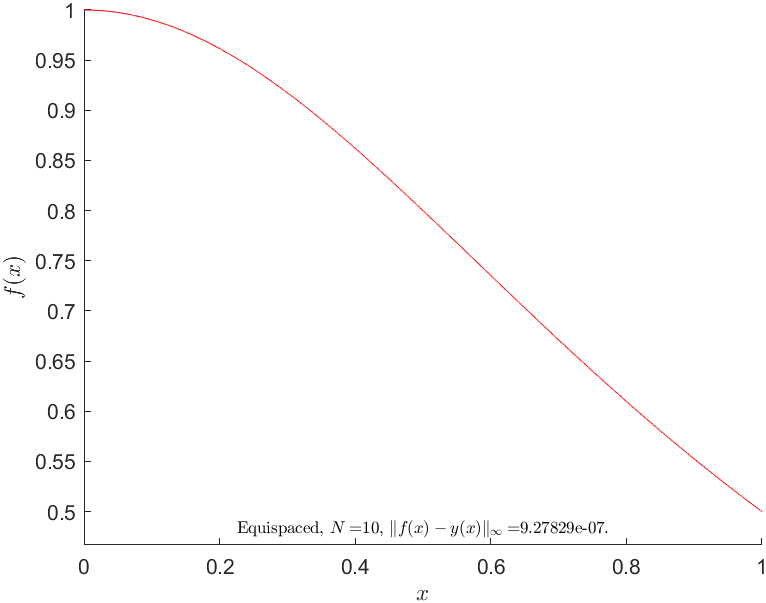
\includegraphics[width=1.0\linewidth]{LagrangeHermit/Lagr_Equi_F1_N10.png}}
		\end{minipage}%
		%\hfill
		\begin{minipage}[h]{0.34\linewidth}
			\center{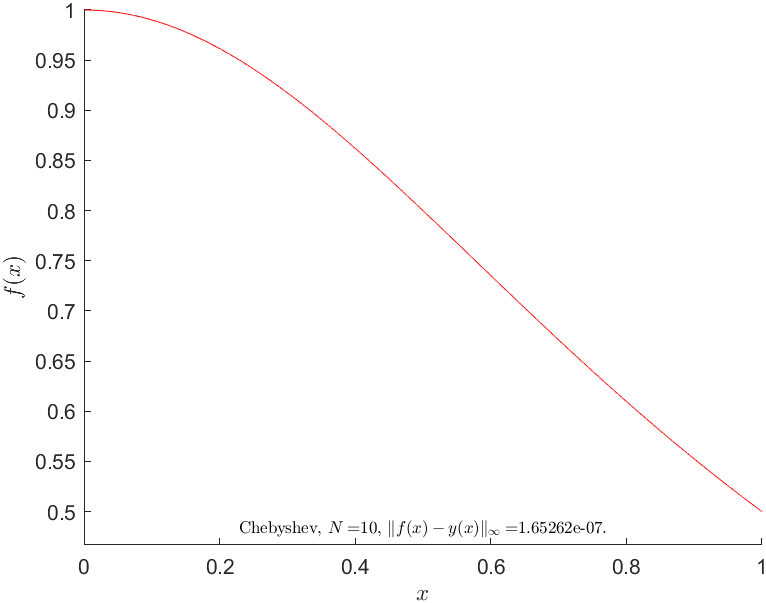
\includegraphics[width=1.0\linewidth]{LagrangeHermit/Lagr_Cheb_F1_N10.png}}
		\end{minipage}%
		%\hfill
		\begin{minipage}[h]{0.34\linewidth}
			\center{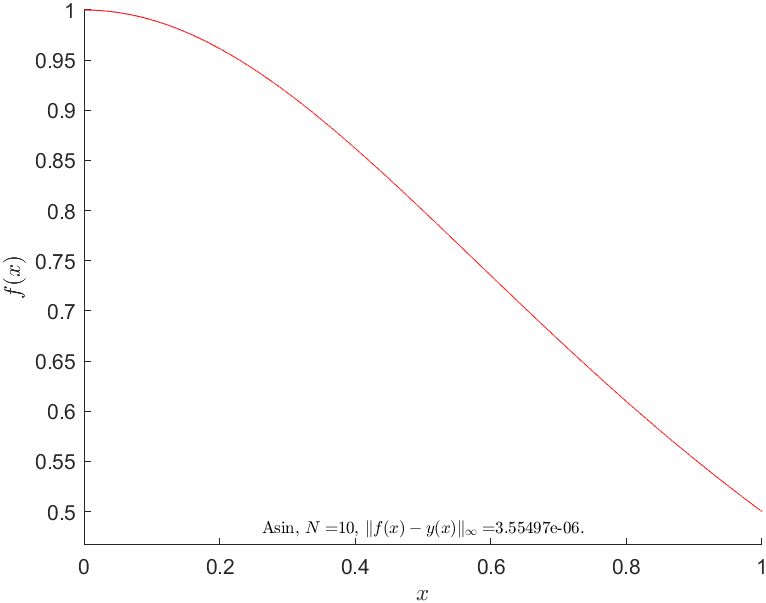
\includegraphics[width=1.0\linewidth]{LagrangeHermit/Lagr_Asin_F1_N10.png}}
		\end{minipage}%
		\vfill
		\begin{minipage}[h]{0.34\linewidth}
			\center{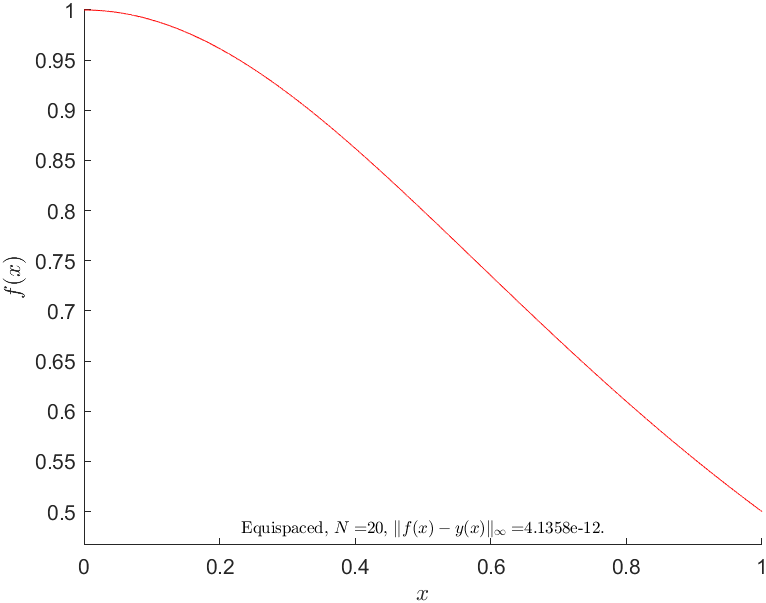
\includegraphics[width=1.0\linewidth]{LagrangeHermit/Lagr_Equi_F1_N20.png}}
		\end{minipage}%
		%\hfill
		\begin{minipage}[h]{0.34\linewidth}
			\center{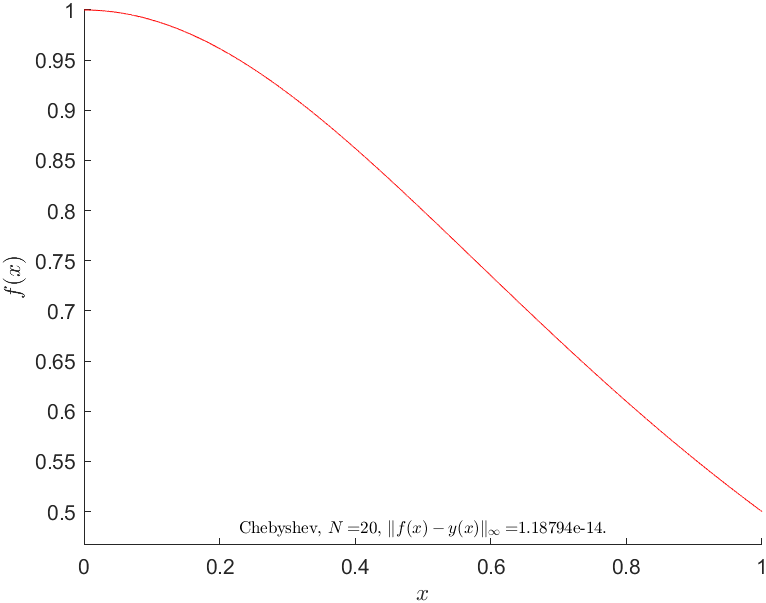
\includegraphics[width=1.0\linewidth]{LagrangeHermit/Lagr_Cheb_F1_N20.png}} 
		\end{minipage}%
		%\hfill
		\begin{minipage}[h]{0.34\linewidth}
			\center{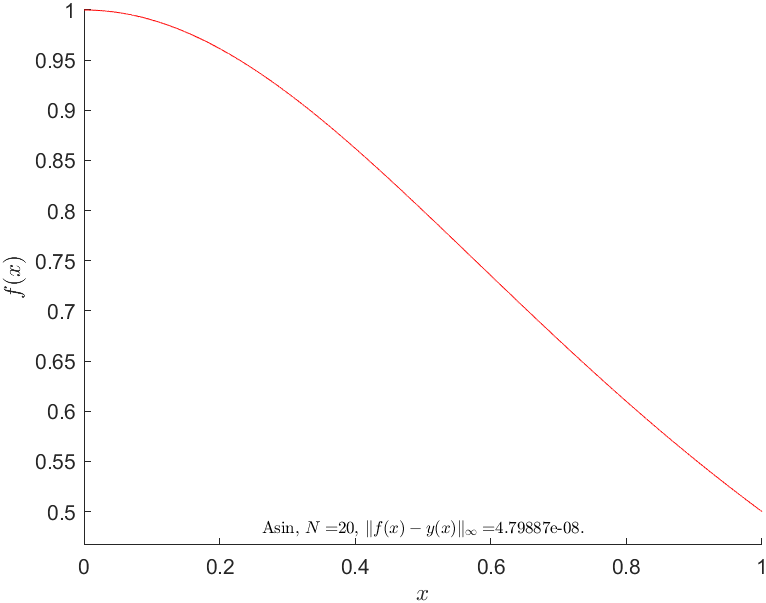
\includegraphics[width=1.0\linewidth]{LagrangeHermit/Lagr_Asin_F1_N20.png}} 
		\end{minipage}%
		\vfill
		\begin{minipage}[h]{0.34\linewidth}
			\center{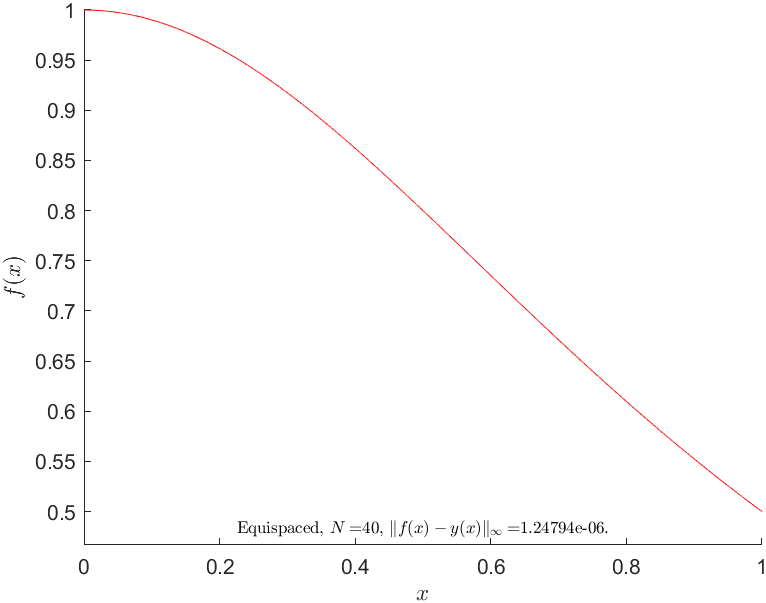
\includegraphics[width=1.0\linewidth]{LagrangeHermit/Lagr_Equi_F1_N40.png}} 
		\end{minipage}%
		%\hfill
		\begin{minipage}[h]{0.34\linewidth}
			\center{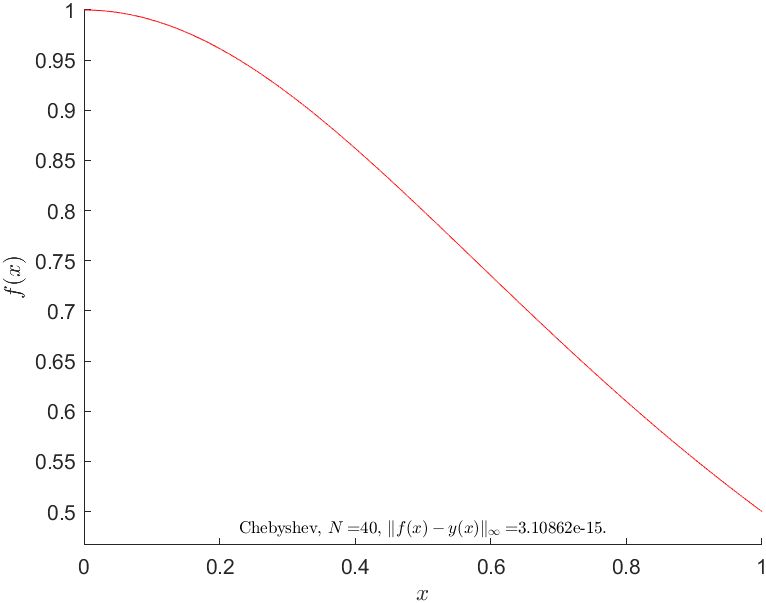
\includegraphics[width=1.0\linewidth]{LagrangeHermit/Lagr_Cheb_F1_N40.png}} 
		\end{minipage}%
		%\hfill
		\begin{minipage}[h]{0.34\linewidth}
			\center{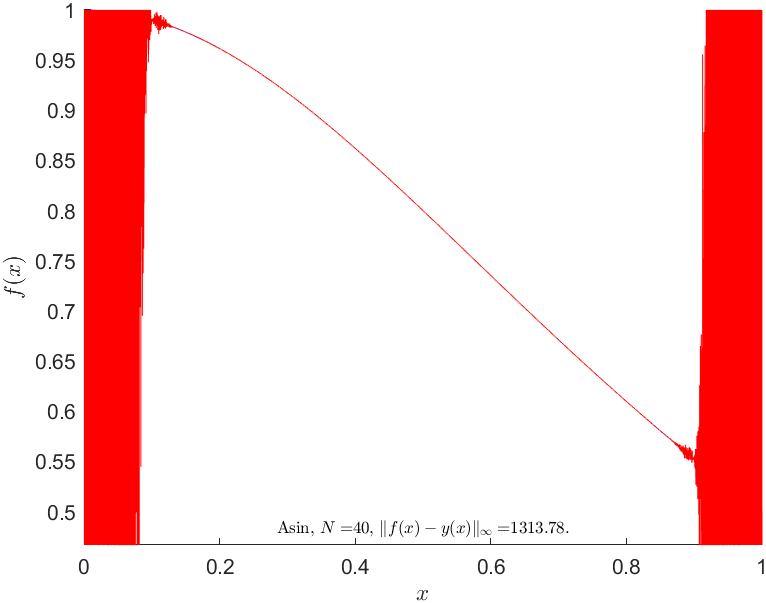
\includegraphics[width=1.0\linewidth]{LagrangeHermit/Lagr_Asin_F1_N40.png}} 
		\end{minipage}%
		\vfill
		\begin{minipage}[h]{0.34\linewidth}
			\center{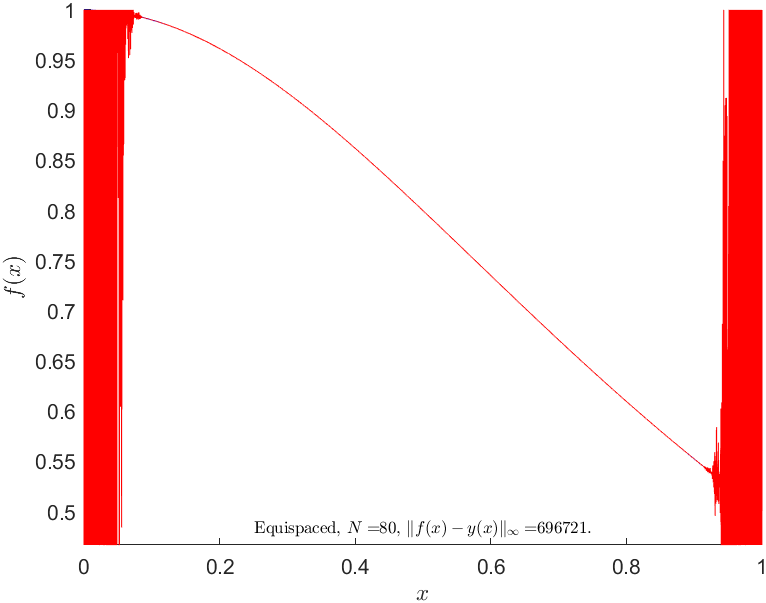
\includegraphics[width=1.0\linewidth]{LagrangeHermit/Lagr_Equi_F1_N80.png}} 
		\end{minipage}%
		%\hfill
		\begin{minipage}[h]{0.34\linewidth}
			\center{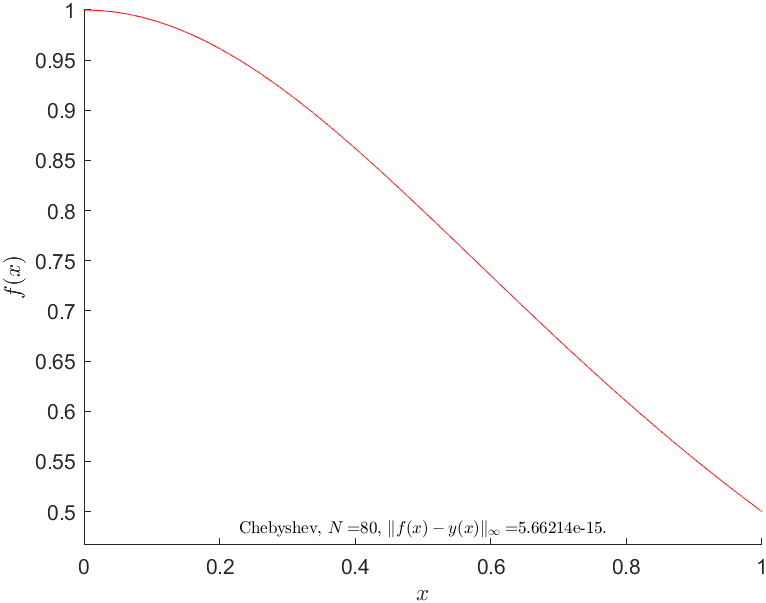
\includegraphics[width=1.0\linewidth]{LagrangeHermit/Lagr_Cheb_F1_N80.png}} 
		\end{minipage}%
		%\hfill
		\begin{minipage}[h]{0.34\linewidth}
			\center{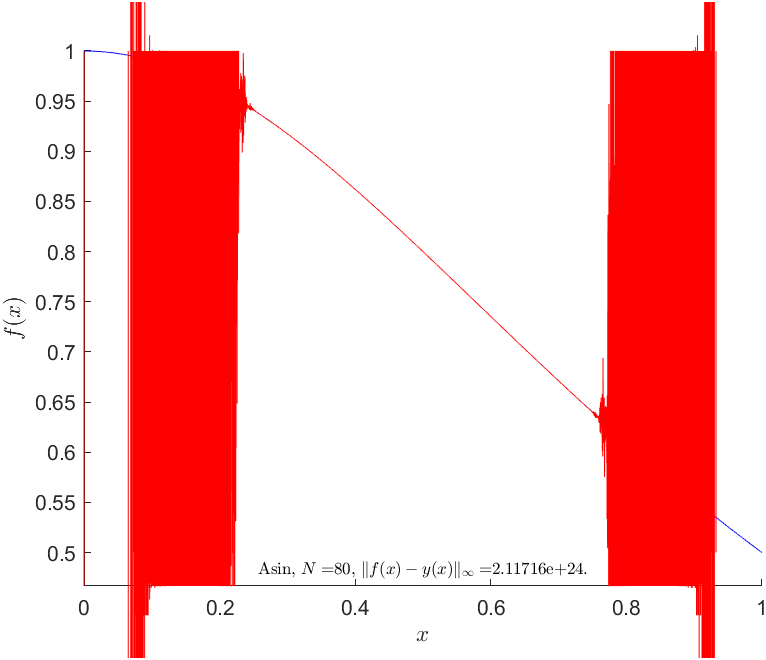
\includegraphics[width=1.0\linewidth]{LagrangeHermit/Lagr_Asin_F1_N80.png}} 
		\end{minipage}%
		\caption{Results of Lagrange interpolation for 10, 20, 40 and 80 data points. The function is pictured with blue, its interpolant with red. First colomn corresponds to Equispaced data point distribution, second to Chebyshev and third to Asin.}
		%\label{ris:Area1-5}
	\end{figure}
\newpage
	\subsection{Hermit interpolant}
		\begin{figure}[H]
		\begin{minipage}[h]{0.34\linewidth}
			\center{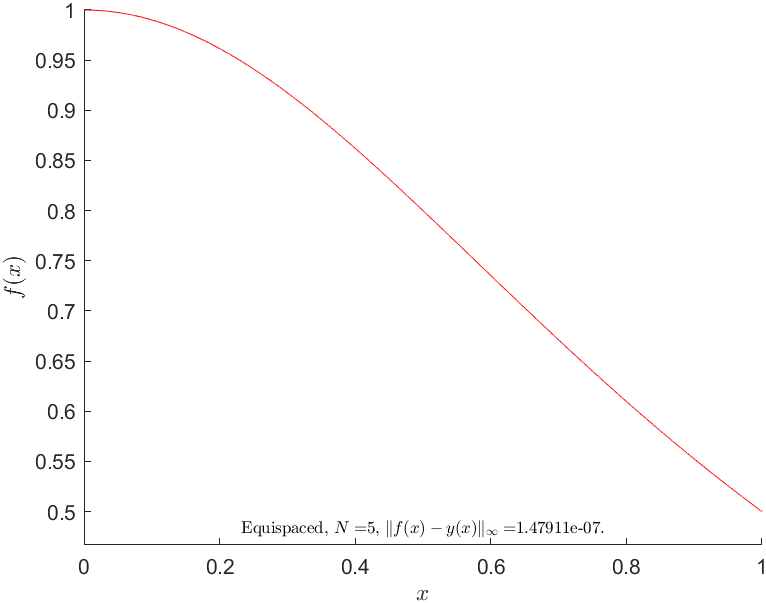
\includegraphics[width=1.0\linewidth]{LagrangeHermit/Herm_Equi_F1_N5.png}}
		\end{minipage}%
		%\hfill
		\begin{minipage}[h]{0.34\linewidth}
			\center{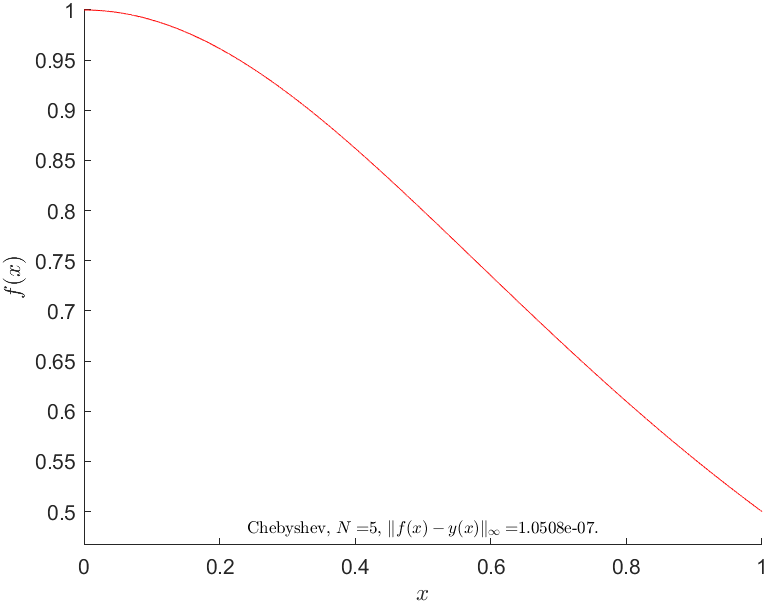
\includegraphics[width=1.0\linewidth]{LagrangeHermit/Herm_Cheb_F1_N5.png}}
		\end{minipage}%
		%\hfill
		\begin{minipage}[h]{0.34\linewidth}
			\center{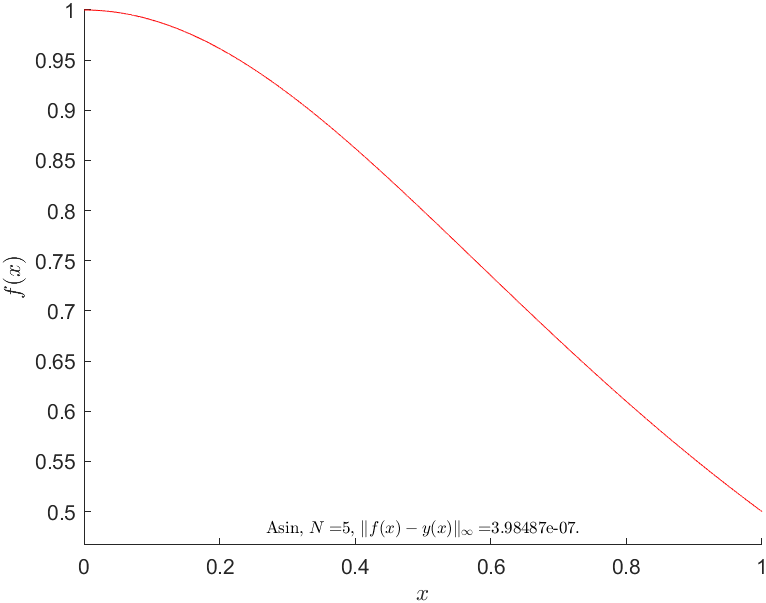
\includegraphics[width=1.0\linewidth]{LagrangeHermit/Herm_Asin_F1_N5.png}}
		\end{minipage}%
		\vfill
		\begin{minipage}[h]{0.34\linewidth}
			\center{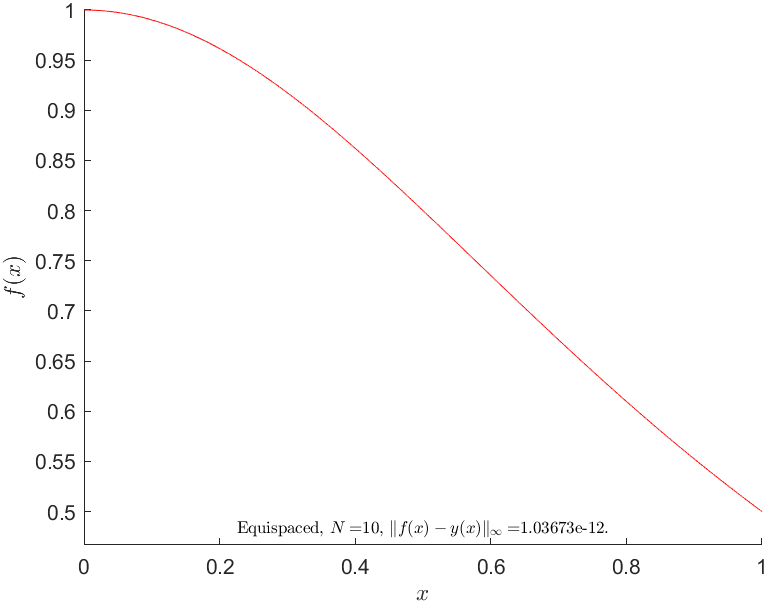
\includegraphics[width=1.0\linewidth]{LagrangeHermit/Herm_Equi_F1_N10.png}}
		\end{minipage}%
		%\hfill
		\begin{minipage}[h]{0.34\linewidth}
			\center{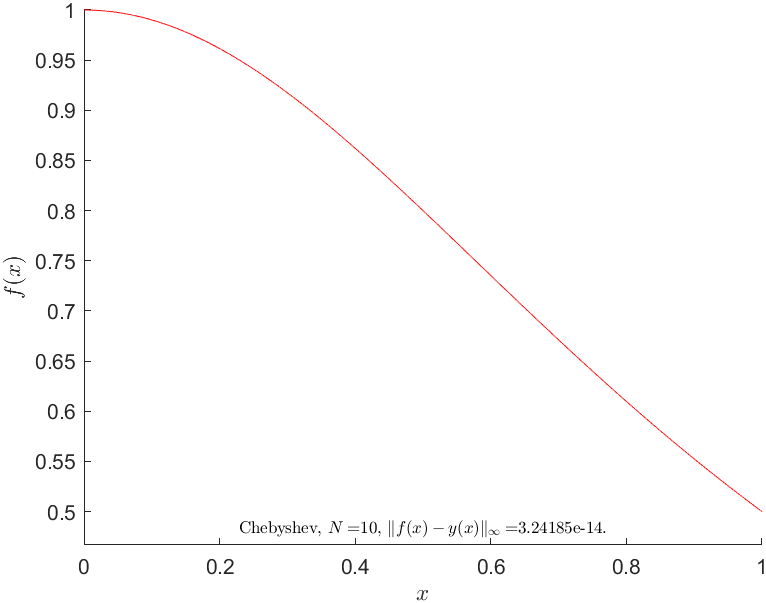
\includegraphics[width=1.0\linewidth]{LagrangeHermit/Herm_Cheb_F1_N10.png}} 
		\end{minipage}%
		%\hfill
		\begin{minipage}[h]{0.34\linewidth}
			\center{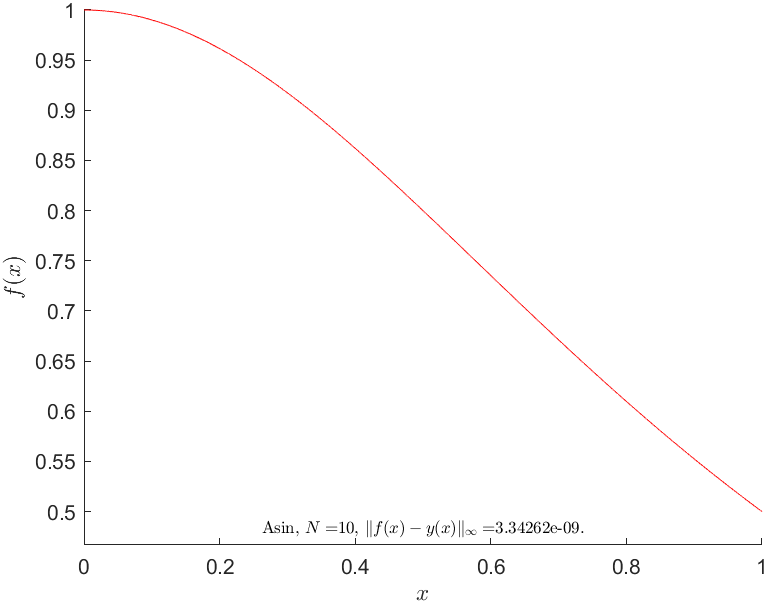
\includegraphics[width=1.0\linewidth]{LagrangeHermit/Herm_Asin_F1_N10.png}} 
		\end{minipage}%
		\vfill
		\begin{minipage}[h]{0.34\linewidth}
			\center{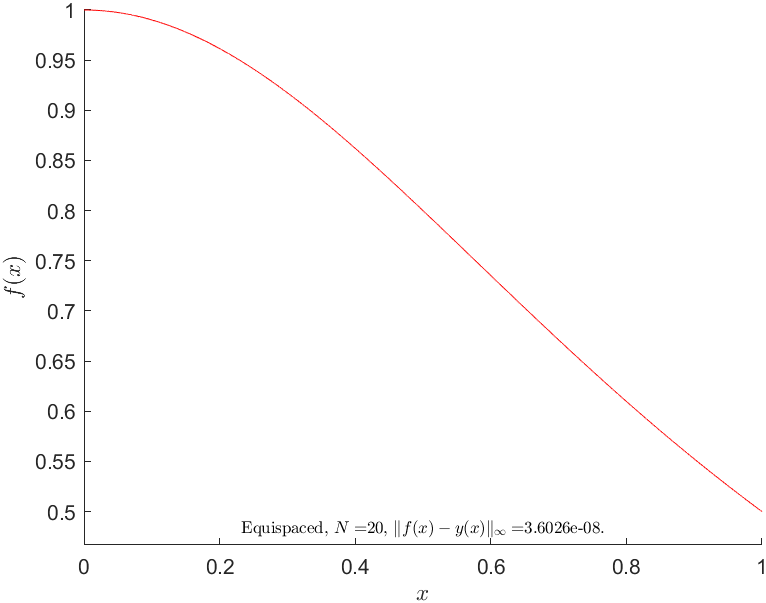
\includegraphics[width=1.0\linewidth]{LagrangeHermit/Herm_Equi_F1_N20.png}} 
		\end{minipage}%
		%\hfill
		\begin{minipage}[h]{0.34\linewidth}
			\center{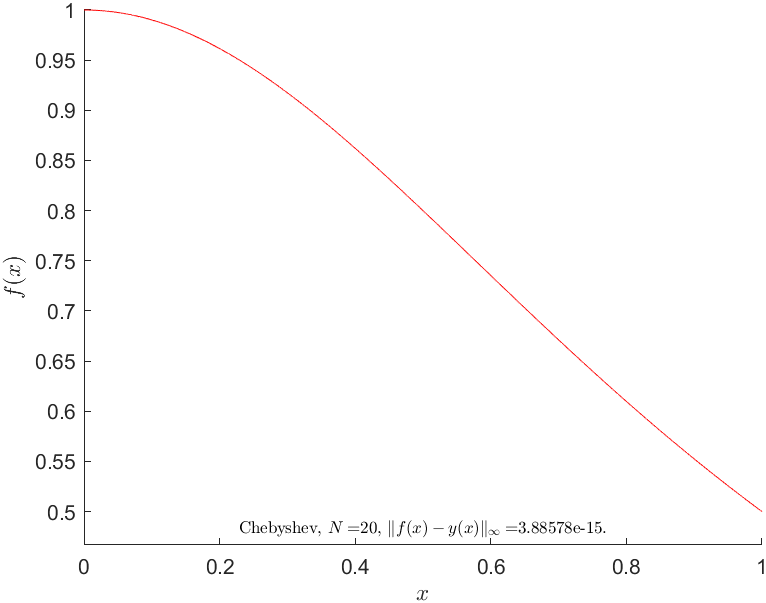
\includegraphics[width=1.0\linewidth]{LagrangeHermit/Herm_Cheb_F1_N20.png}} 
		\end{minipage}%
		%\hfill
		\begin{minipage}[h]{0.34\linewidth}
			\center{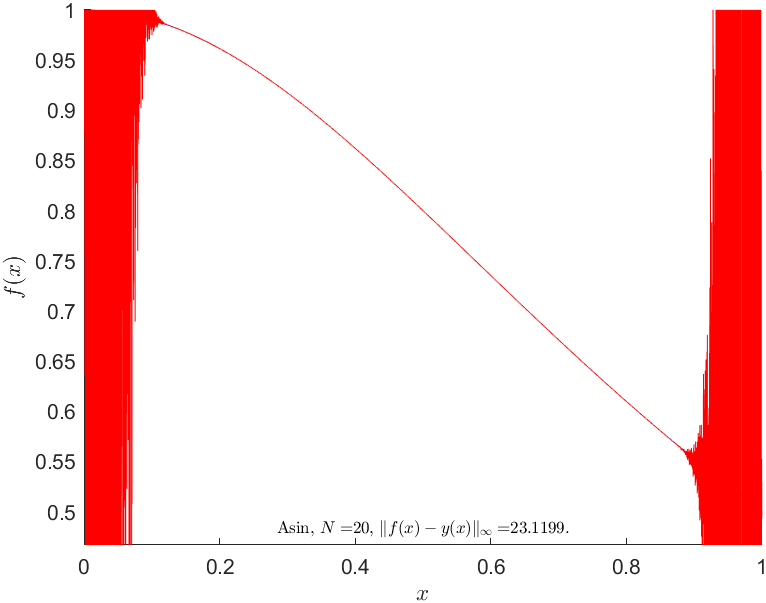
\includegraphics[width=1.0\linewidth]{LagrangeHermit/Herm_Asin_F1_N20.png}} 
		\end{minipage}%
		\vfill
		\begin{minipage}[h]{0.34\linewidth}
			\center{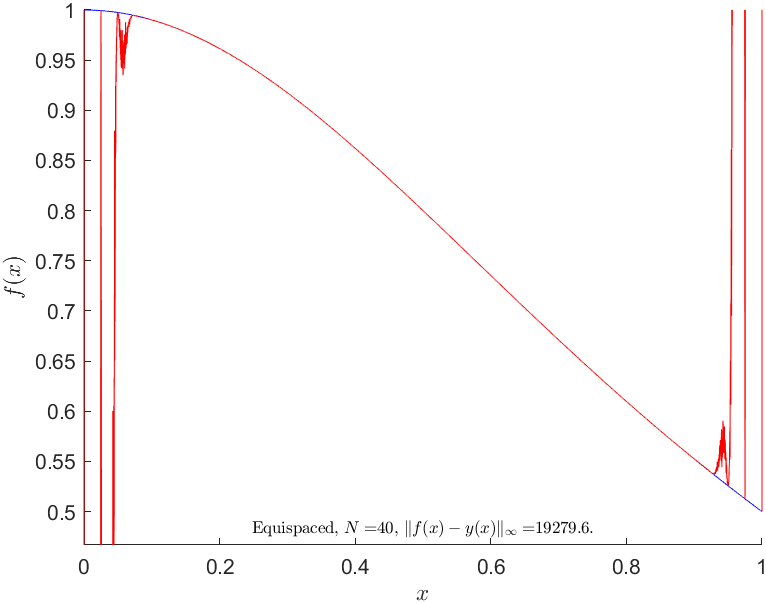
\includegraphics[width=1.0\linewidth]{LagrangeHermit/Herm_Equi_F1_N40.png}} 
		\end{minipage}%
		%\hfill
		\begin{minipage}[h]{0.34\linewidth}
			\center{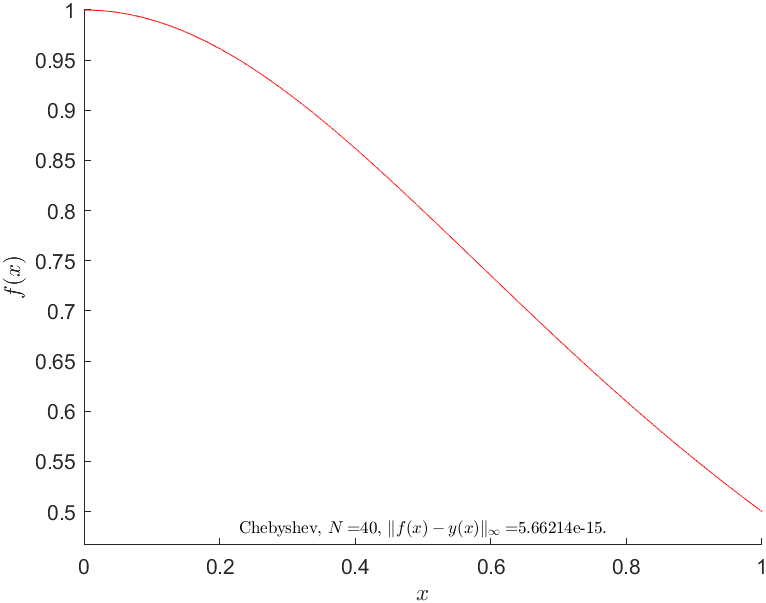
\includegraphics[width=1.0\linewidth]{LagrangeHermit/Herm_Cheb_F1_N40.png}} 
		\end{minipage}%
		%\hfill
		\begin{minipage}[h]{0.34\linewidth}
			\center{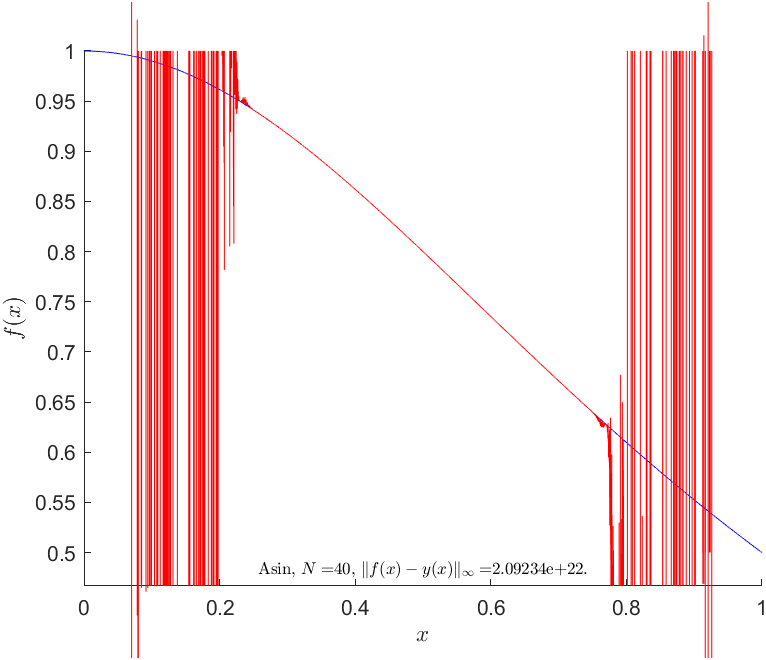
\includegraphics[width=1.0\linewidth]{LagrangeHermit/Herm_Asin_F1_N40.png}} 
		\end{minipage}%
		\caption{Results of Hermit interpolation for 5, 10, 20 and 40 data points. The function is pictured with blue, its interpolant with red. First colomn corresponds to Equispaced data point distribution, second to Chebyshev and third to Asin.}
		%\label{ris:Area1-5}
	\end{figure}
	\newpage
	\subsection{Accuracy analysis}
		\begin{figure}[H]
		\begin{minipage}[h]{0.5\linewidth}
			\center{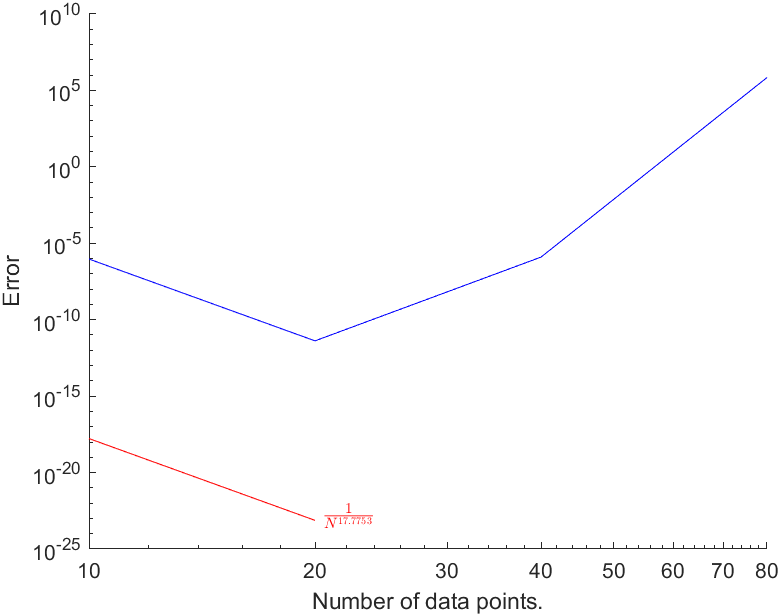
\includegraphics[width=1.0\linewidth]{LagrangeHermit/Lagr_eq_err_F1.png}}
			\caption{Dependence of error on the number of data\\ points for Lagrange interpolant and Equispaced point distribution.}
		\end{minipage}%
		\hspace{0.5cm}
		%\hfill
		\begin{minipage}[h]{0.5\linewidth}
			\center{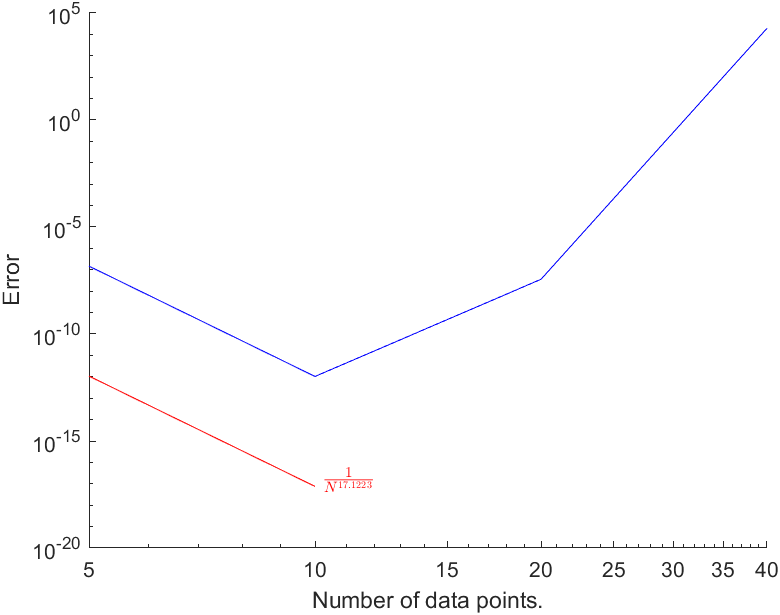
\includegraphics[width=1.0\linewidth]{LagrangeHermit/Herm_eq_err_F1.png}} 
			\caption{Dependence of error on the number of data\\ points for Hermit interpolant and Equispaced point distribution.}
		\end{minipage}%
		\vfill
		\begin{minipage}[h]{0.5\linewidth}
			\center{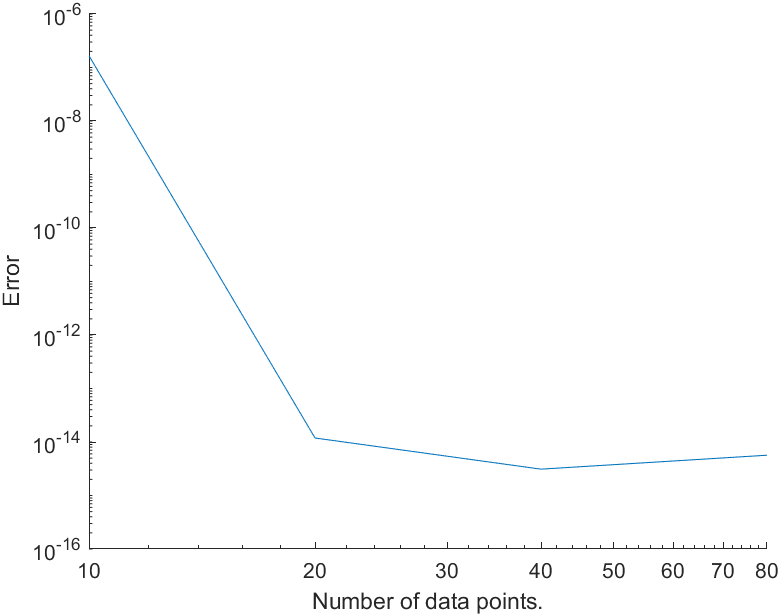
\includegraphics[width=1.0\linewidth]{LagrangeHermit/Lagr_cheb_err_F1.png}} 
			\caption{Dependence of error on the number of data\\ points for Lagrange interpolant and Chebyshev point distribution.}
		\end{minipage}%
	\hspace{0.5cm}
		%\hfill
		\begin{minipage}[h]{0.5\linewidth}
			\center{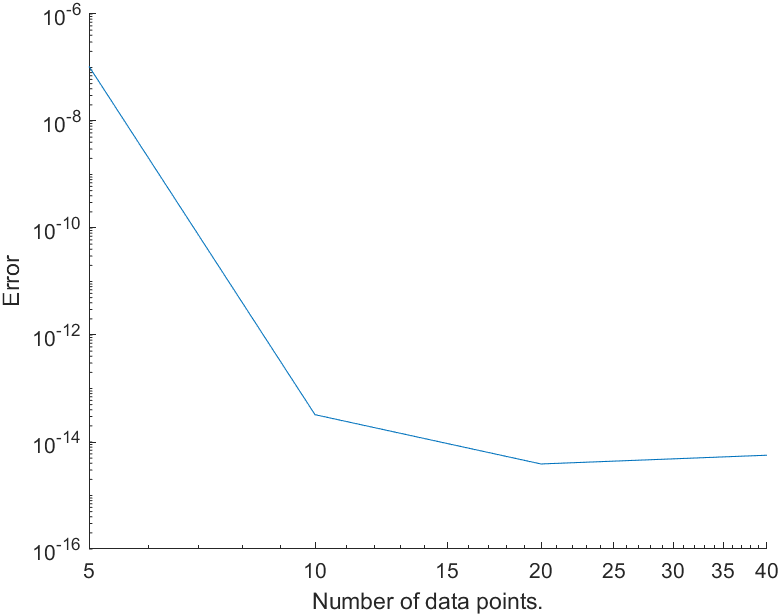
\includegraphics[width=1.0\linewidth]{LagrangeHermit/Herm_cheb_err_F1.png}} 
				\caption{Dependence of error on the number of data\\ points for Hermit interpolant and Chebyshev point distribution.}
		\end{minipage}%
		%\hfill
		\vfill
		\begin{minipage}[h]{0.5\linewidth}
			\center{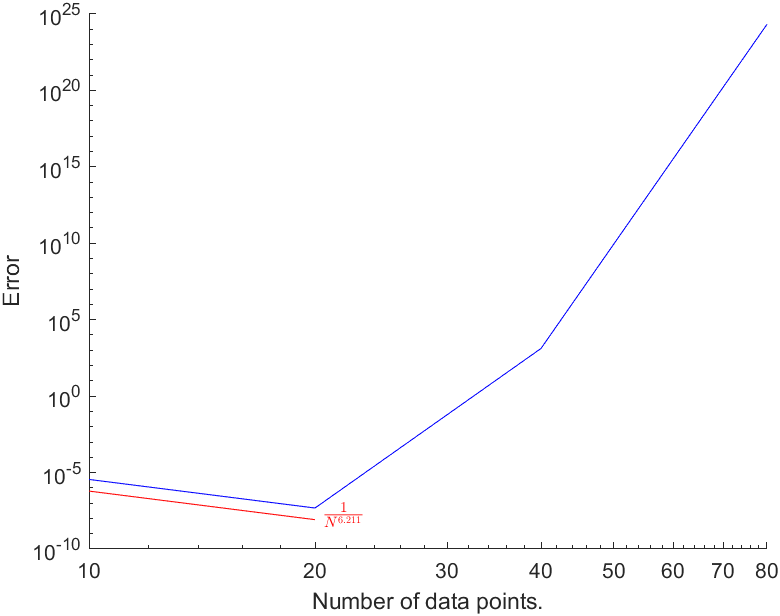
\includegraphics[width=1.0\linewidth]{LagrangeHermit/Lagr_asin_err_F1.png}} 
				\caption{Dependence of error on the number of data\\ points for Lagrange interpolant and Asin point distribution.}
		\end{minipage}%
	\hspace{0.5cm}
		%\hfill
		\begin{minipage}[h]{0.5\linewidth}
			\center{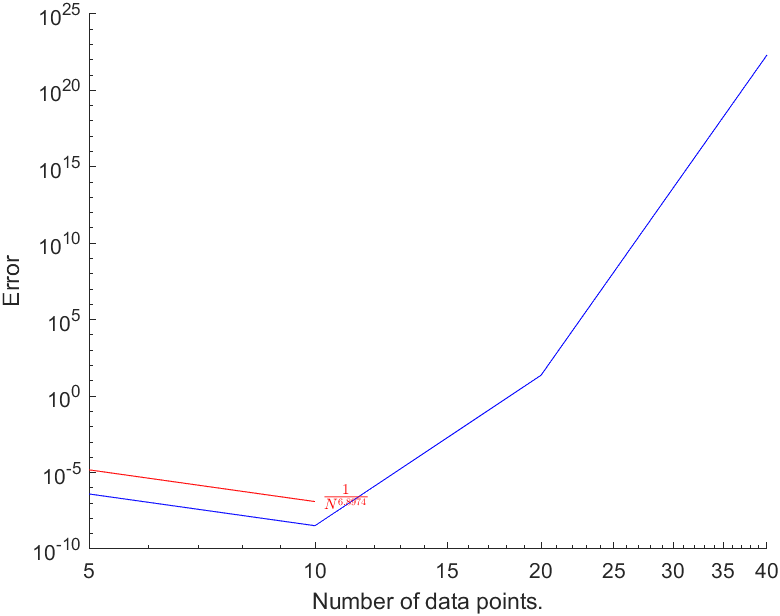
\includegraphics[width=1.0\linewidth]{LagrangeHermit/Herm_asin_err_F1.png}} 
			\caption{Dependence of error on the number of data\\ points for Hermit interpolant and Asin point distribution.}
		\end{minipage}%
		%\hfill
	\end{figure}

As expected, Chebyshev point distribution provides the best accuracy. Second best is for Equispaced distribution and the worst is for Asin. Since Chebyshev point distribution is the most accurate and it gets denser the closer the interval boundaries are, it seems logical that Asin is the least accurate, because it gets rarer when approaching them. For this particular function Hermit interpolation turned out to be more accurate than Lagrange. Most likely it is due to the function smoothness. Note that for high $N$ the error grows rapidly, which is not only connected with $\|y^{N+1}\|$ growth, but also with "round-off" error accumulation.  
	\newpage
	
	%%%%%%%%%%%%%%%2
		\section{$ (x-\frac{1}{2})^2 sign(x-\frac{1}{2}) $}
	\subsection{Lagrange interpolant}
	\begin{figure}[H]
		\begin{minipage}[h]{0.34\linewidth}
			\center{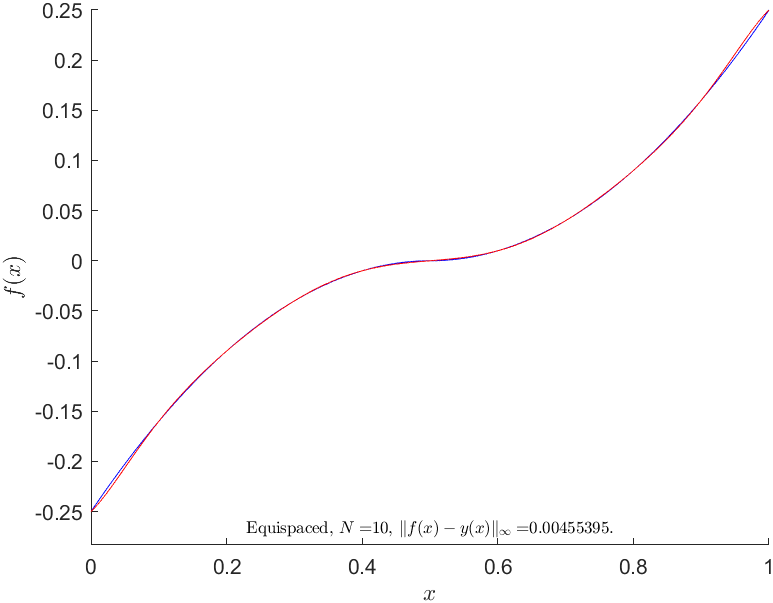
\includegraphics[width=1.0\linewidth]{LagrangeHermit/Lagr_Equi_F2_N10.png}}
		\end{minipage}%
		%\hfill
		\begin{minipage}[h]{0.34\linewidth}
			\center{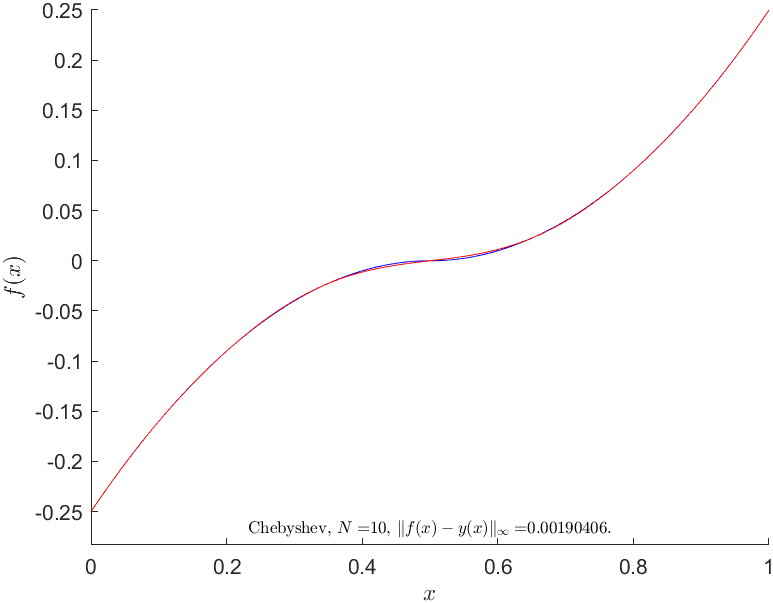
\includegraphics[width=1.0\linewidth]{LagrangeHermit/Lagr_Cheb_F2_N10.png}}
		\end{minipage}%
		%\hfill
		\begin{minipage}[h]{0.34\linewidth}
			\center{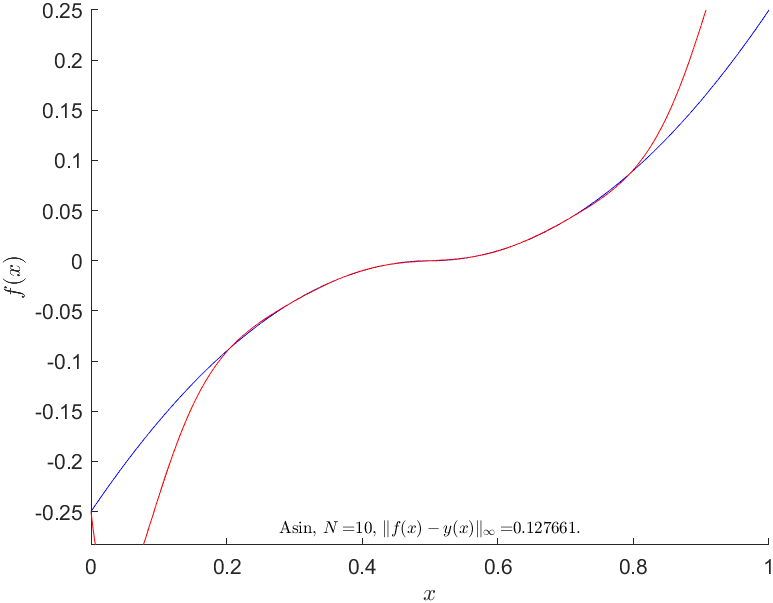
\includegraphics[width=1.0\linewidth]{LagrangeHermit/Lagr_Asin_F2_N10.png}}
		\end{minipage}%
		\vfill
		\begin{minipage}[h]{0.34\linewidth}
			\center{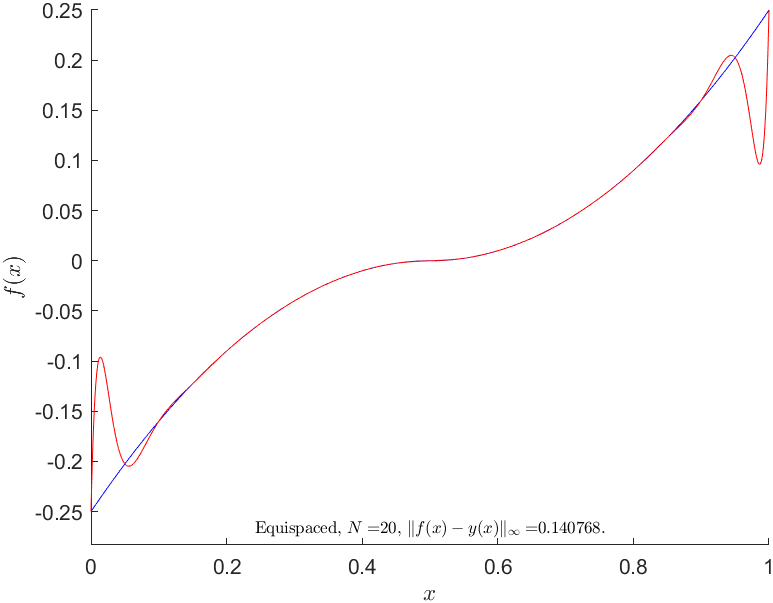
\includegraphics[width=1.0\linewidth]{LagrangeHermit/Lagr_Equi_F2_N20.png}}
		\end{minipage}%
		%\hfill
		\begin{minipage}[h]{0.34\linewidth}
			\center{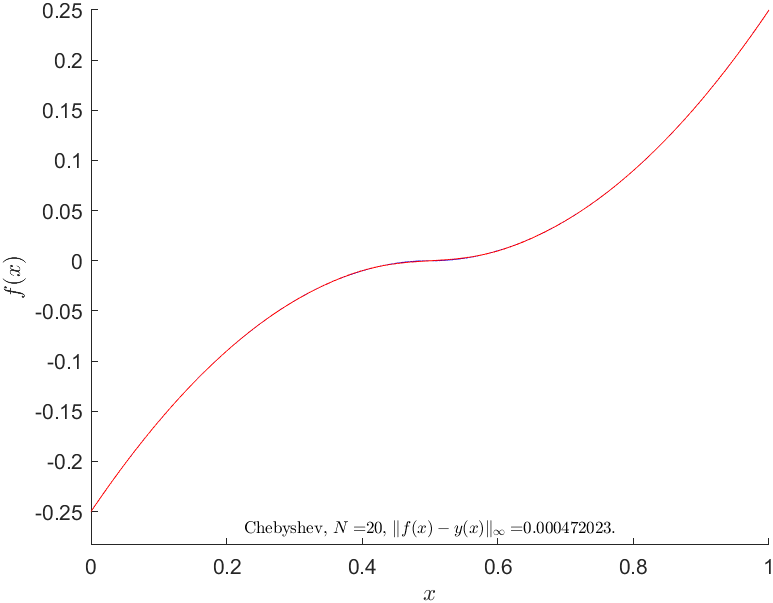
\includegraphics[width=1.0\linewidth]{LagrangeHermit/Lagr_Cheb_F2_N20.png}} 
		\end{minipage}%
		%\hfill
		\begin{minipage}[h]{0.34\linewidth}
			\center{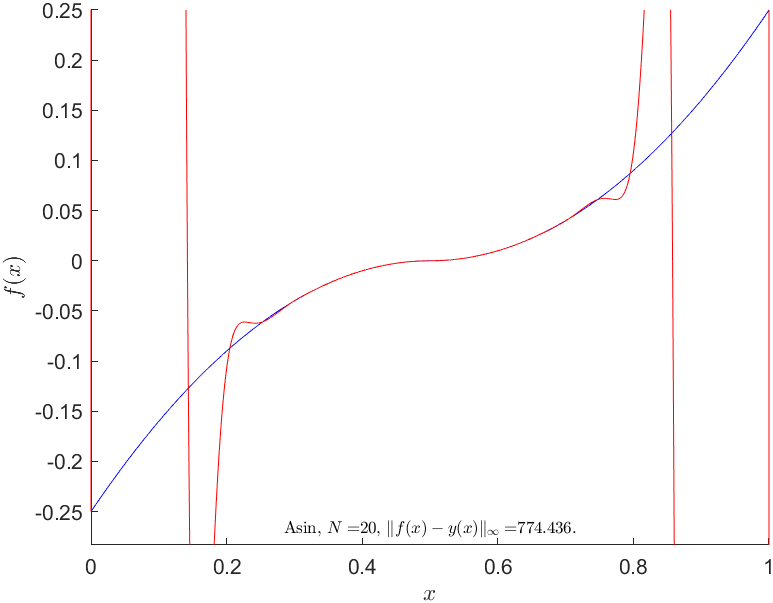
\includegraphics[width=1.0\linewidth]{LagrangeHermit/Lagr_Asin_F2_N20.png}} 
		\end{minipage}%
		\vfill
		\begin{minipage}[h]{0.34\linewidth}
			\center{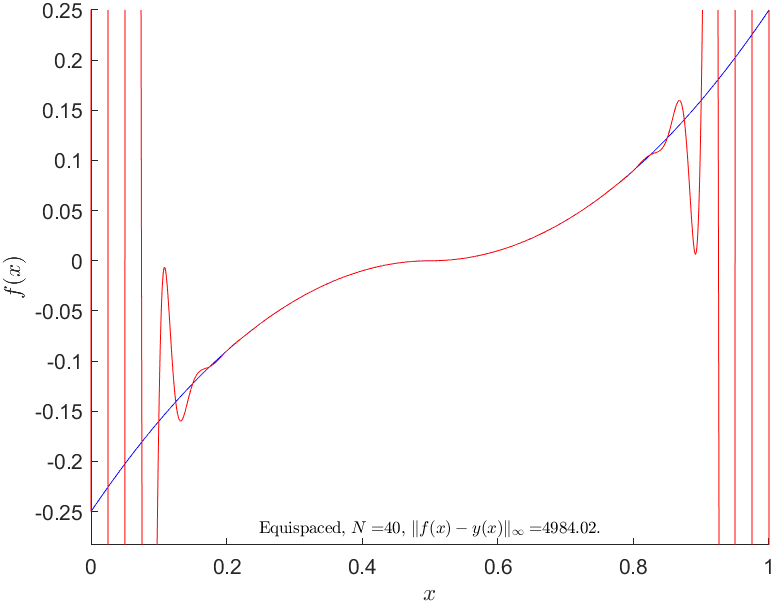
\includegraphics[width=1.0\linewidth]{LagrangeHermit/Lagr_Equi_F2_N40.png}} 
		\end{minipage}%
		%\hfill
		\begin{minipage}[h]{0.34\linewidth}
			\center{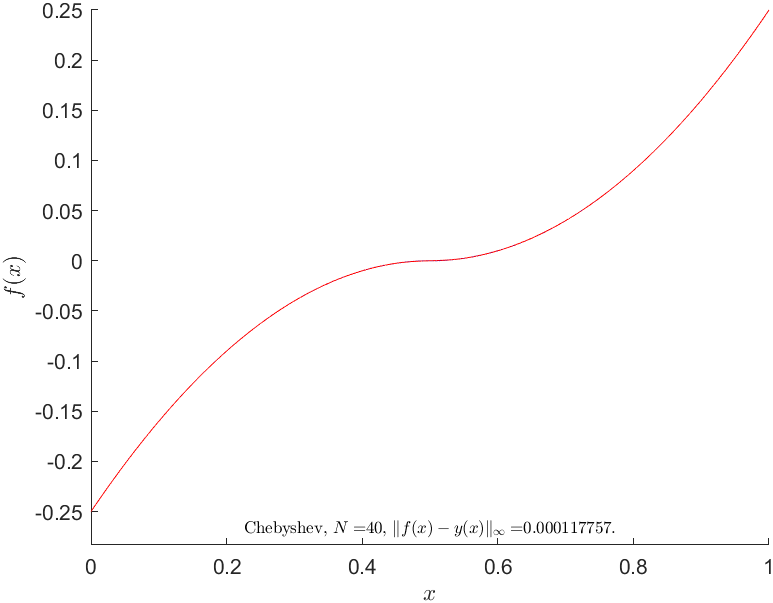
\includegraphics[width=1.0\linewidth]{LagrangeHermit/Lagr_Cheb_F2_N40.png}} 
		\end{minipage}%
		%\hfill
		\begin{minipage}[h]{0.34\linewidth}
			\center{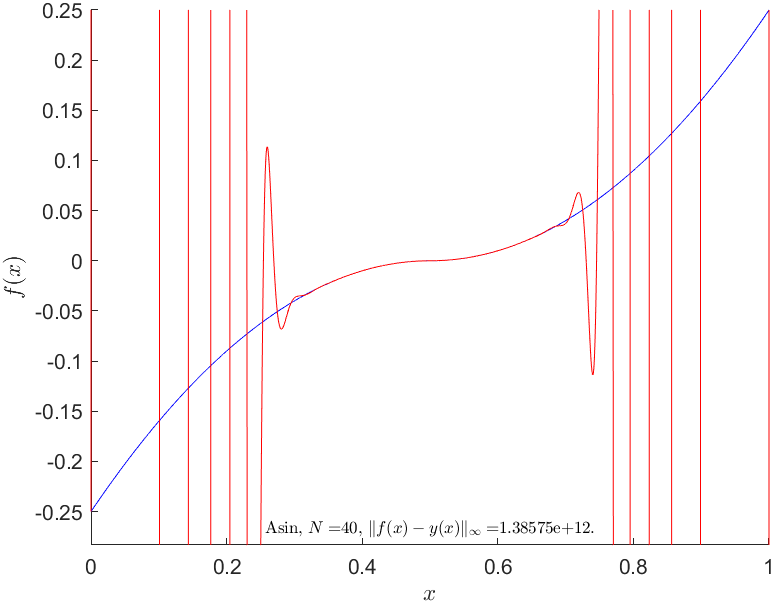
\includegraphics[width=1.0\linewidth]{LagrangeHermit/Lagr_Asin_F2_N40.png}} 
		\end{minipage}%
		\vfill
		\begin{minipage}[h]{0.34\linewidth}
			\center{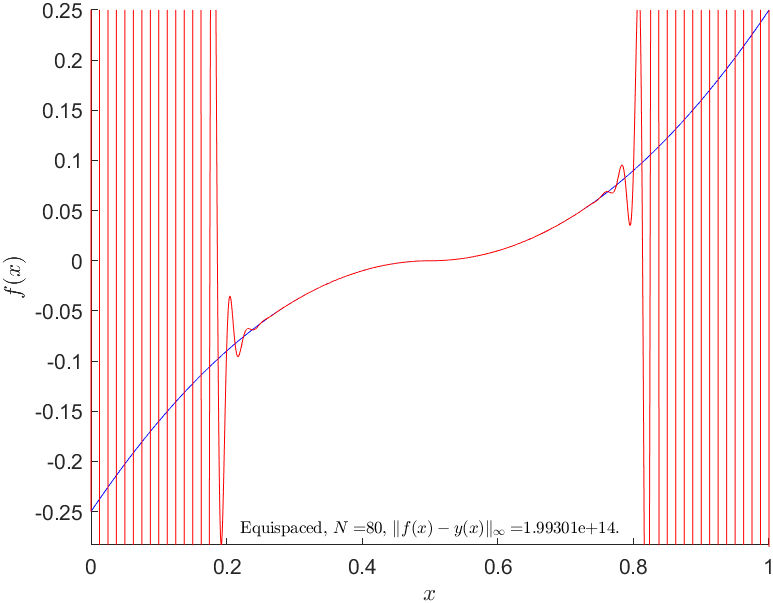
\includegraphics[width=1.0\linewidth]{LagrangeHermit/Lagr_Equi_F2_N80.png}} 
		\end{minipage}%
		%\hfill
		\begin{minipage}[h]{0.34\linewidth}
			\center{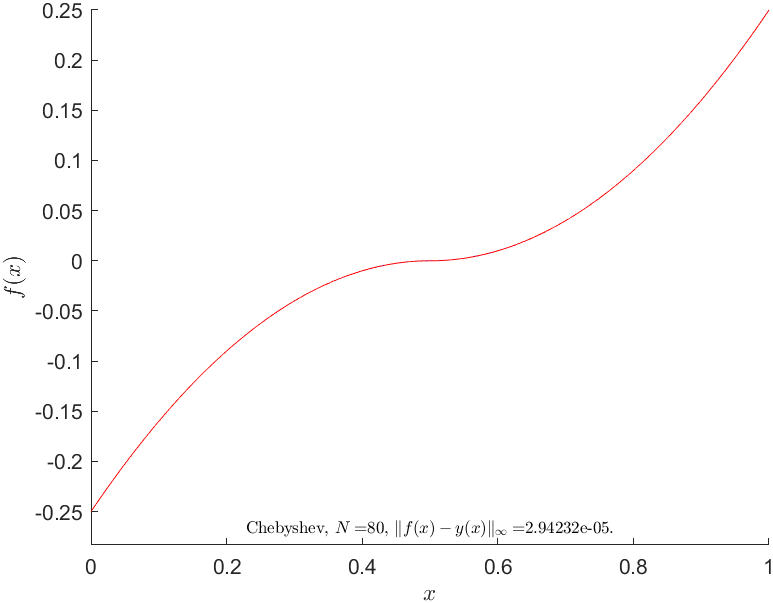
\includegraphics[width=1.0\linewidth]{LagrangeHermit/Lagr_Cheb_F2_N80.png}} 
		\end{minipage}%
		%\hfill
		\begin{minipage}[h]{0.34\linewidth}
			\center{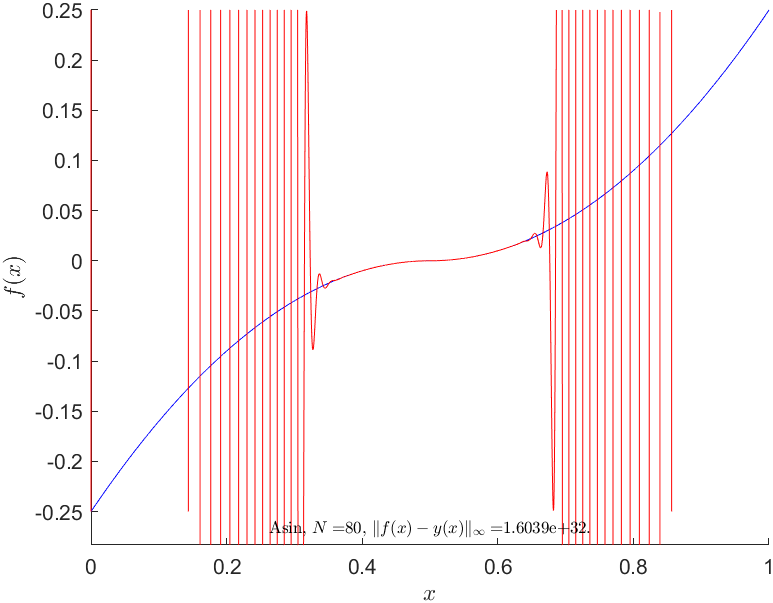
\includegraphics[width=1.0\linewidth]{LagrangeHermit/Lagr_Asin_F2_N80.png}} 
		\end{minipage}%
		\caption{Results of Lagrange interpolation for 10, 20, 40 and 80 data points. The function is pictured with blue, its interpolant with red. First colomn corresponds to Equispaced data point distribution, second to Chebyshev and third to Asin.}
		%\label{ris:Area1-5}
	\end{figure}
	\newpage
	\subsection{Hermit interpolant}
	\begin{figure}[H]
		\begin{minipage}[h]{0.34\linewidth}
			\center{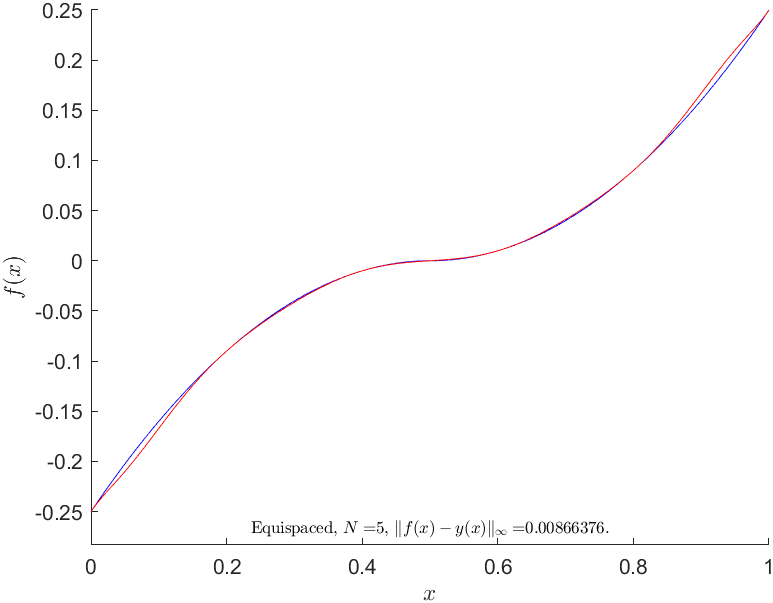
\includegraphics[width=1.0\linewidth]{LagrangeHermit/Herm_Equi_F2_N5.png}}
		\end{minipage}%
		%\hfill
		\begin{minipage}[h]{0.34\linewidth}
			\center{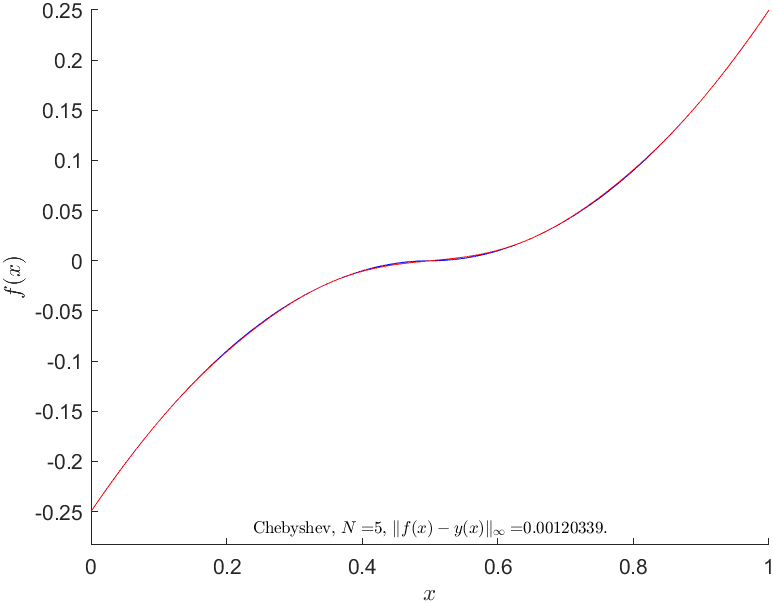
\includegraphics[width=1.0\linewidth]{LagrangeHermit/Herm_Cheb_F2_N5.png}}
		\end{minipage}%
		%\hfill
		\begin{minipage}[h]{0.34\linewidth}
			\center{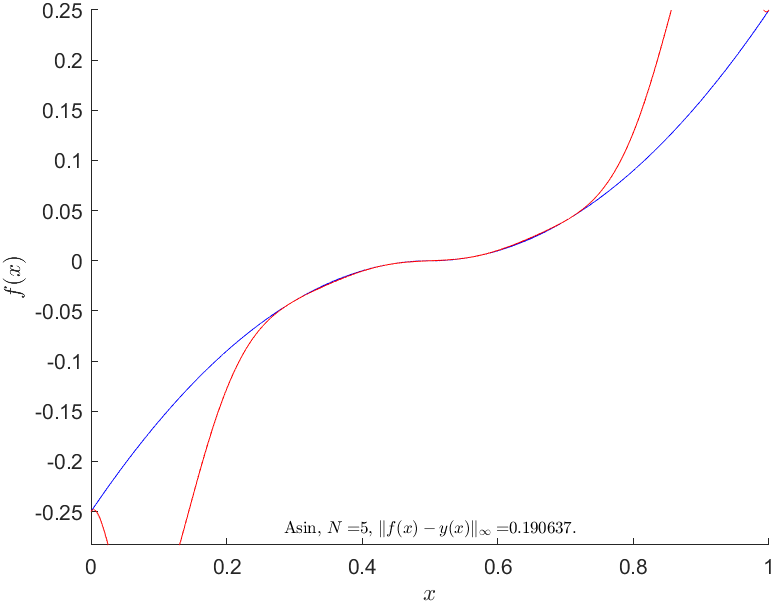
\includegraphics[width=1.0\linewidth]{LagrangeHermit/Herm_Asin_F2_N5.png}}
		\end{minipage}%
		\vfill
		\begin{minipage}[h]{0.34\linewidth}
			\center{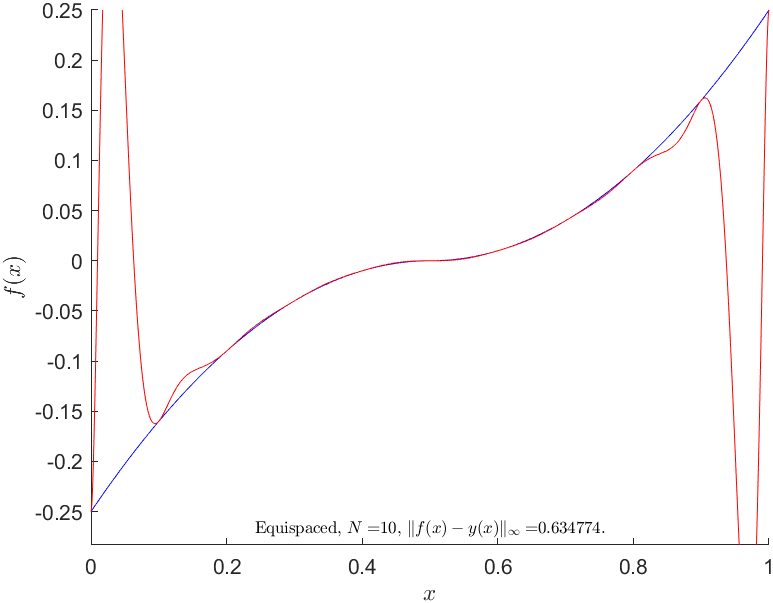
\includegraphics[width=1.0\linewidth]{LagrangeHermit/Herm_Equi_F2_N10.png}}
		\end{minipage}%
		%\hfill
		\begin{minipage}[h]{0.34\linewidth}
			\center{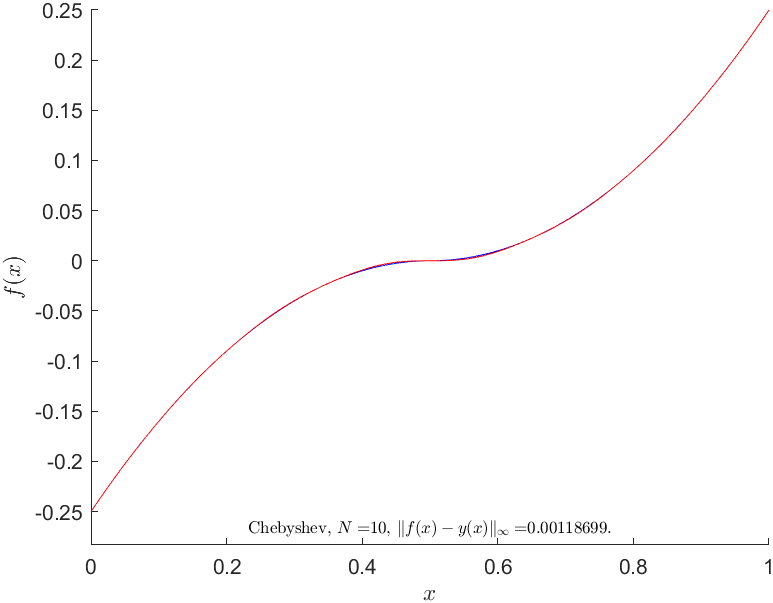
\includegraphics[width=1.0\linewidth]{LagrangeHermit/Herm_Cheb_F2_N10.png}} 
		\end{minipage}%
		%\hfill
		\begin{minipage}[h]{0.34\linewidth}
			\center{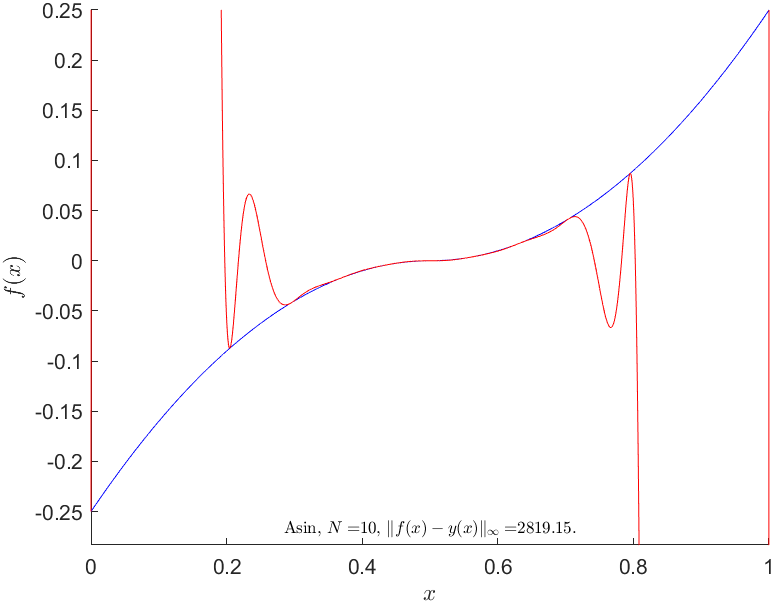
\includegraphics[width=1.0\linewidth]{LagrangeHermit/Herm_Asin_F2_N10.png}} 
		\end{minipage}%
		\vfill
		\begin{minipage}[h]{0.34\linewidth}
			\center{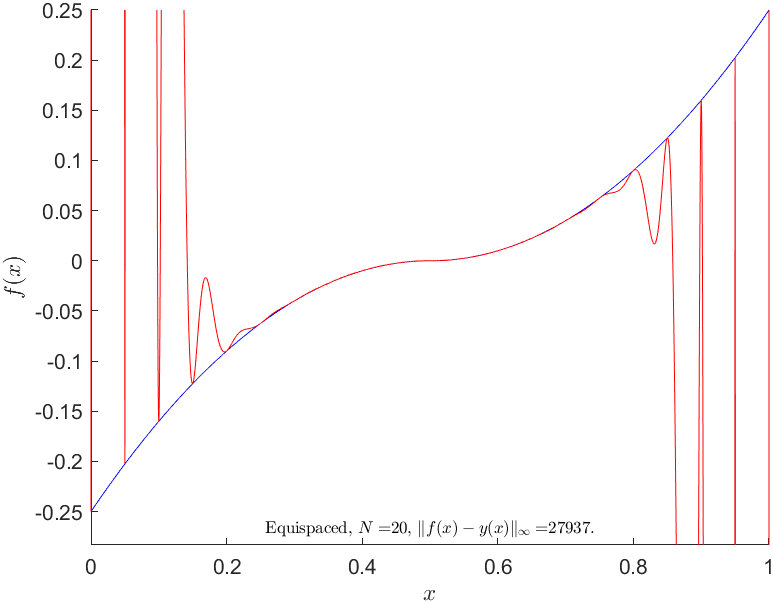
\includegraphics[width=1.0\linewidth]{LagrangeHermit/Herm_Equi_F2_N20.png}} 
		\end{minipage}%
		%\hfill
		\begin{minipage}[h]{0.34\linewidth}
			\center{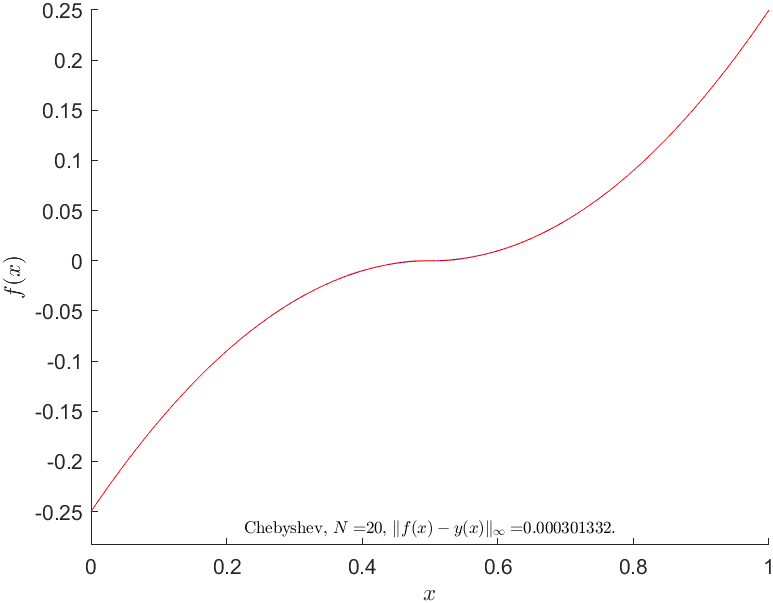
\includegraphics[width=1.0\linewidth]{LagrangeHermit/Herm_Cheb_F2_N20.png}} 
		\end{minipage}%
		%\hfill
		\begin{minipage}[h]{0.34\linewidth}
			\center{\includegraphics[width=1.0\linewidth]{LagrangeHermit/Herm_Asin_F2_N20.png}} 
		\end{minipage}%
		\vfill
		\begin{minipage}[h]{0.34\linewidth}
			\center{\includegraphics[width=1.0\linewidth]{LagrangeHermit/Herm_Equi_F2_N40.png}} 
		\end{minipage}%
		%\hfill
		\begin{minipage}[h]{0.34\linewidth}
			\center{\includegraphics[width=1.0\linewidth]{LagrangeHermit/Herm_Cheb_F2_N40.png}} 
		\end{minipage}%
		%\hfill
		\begin{minipage}[h]{0.34\linewidth}
			\center{\includegraphics[width=1.0\linewidth]{LagrangeHermit/Herm_Asin_F2_N40.png}} 
		\end{minipage}%
		\caption{Results of Hermit interpolation for 5, 10, 20 and 40 data points. The function is pictured with blue, its interpolant with red. First colomn corresponds to Equispaced data point distribution, second to Chebyshev and third to Asin.}
		%\label{ris:Area1-5}
	\end{figure}
	\newpage
	\subsection{Accuracy analysis}
	\begin{figure}[H]
		\begin{minipage}[h]{0.45\linewidth}
			\center{\includegraphics[width=1.0\linewidth]{LagrangeHermit/Lagr_eq_err_F2.png}}
			\caption{Dependence of error on the number of data\\ points for Lagrange interpolant and Equispaced point distribution.}
		\end{minipage}%
		\hspace{0.5cm}
		%\hfill
		\begin{minipage}[h]{0.45\linewidth}
			\center{\includegraphics[width=1.0\linewidth]{LagrangeHermit/Herm_eq_err_F2.png}} 
			\caption{Dependence of error on the number of data\\ points for Hermit interpolant and Equispaced point distribution.}
		\end{minipage}%
		\vfill
		\begin{minipage}[h]{0.45\linewidth}
			\center{\includegraphics[width=1.0\linewidth]{LagrangeHermit/Lagr_cheb_err_F2.png}} 
			\caption{Dependence of error on the number of data\\ points for Lagrange interpolant and Chebyshev point distribution.}
		\end{minipage}%
		\hspace{0.5cm}
		%\hfill
		\begin{minipage}[h]{0.45\linewidth}
			\center{\includegraphics[width=1.0\linewidth]{LagrangeHermit/Herm_cheb_err_F2.png}} 
			\caption{Dependence of error on the number of data\\ points for Hermit interpolant and Chebyshev point distribution.}
		\end{minipage}%
		%\hfill
		\vfill
		\begin{minipage}[h]{0.45\linewidth}
			\center{\includegraphics[width=1.0\linewidth]{LagrangeHermit/Lagr_asin_err_F2.png}} 
			\caption{Dependence of error on the number of data\\ points for Lagrange interpolant and Asin point distribution.}
		\end{minipage}%
		\hspace{0.5cm}
		%\hfill
		\begin{minipage}[h]{0.45\linewidth}
			\center{\includegraphics[width=1.0\linewidth]{LagrangeHermit/Herm_asin_err_F2.png}} 
			\caption{Dependence of error on the number of data\\ points for Hermit interpolant and Asin point distribution.}
		\end{minipage}%
		%\hfill
	\end{figure}
The accuracy for this function interpolation is significantly smaller. This is because this function is not as smooth as the previous one. For the same reason Lagrange interpolant is more accurate than Hermit.
	\newpage
	
	%%%%%%%%%%%%%%%%%%%3
		\section{$ |x-\frac{1}{2}|  $}
	\subsection{Lagrange interpolant}
	\begin{figure}[H]
		\begin{minipage}[h]{0.34\linewidth}
			\center{\includegraphics[width=1.0\linewidth]{LagrangeHermit/Lagr_Equi_F3_N10.png}}
		\end{minipage}%
		%\hfill
		\begin{minipage}[h]{0.34\linewidth}
			\center{\includegraphics[width=1.0\linewidth]{LagrangeHermit/Lagr_Cheb_F3_N10.png}}
		\end{minipage}%
		%\hfill
		\begin{minipage}[h]{0.34\linewidth}
			\center{\includegraphics[width=1.0\linewidth]{LagrangeHermit/Lagr_Asin_F3_N10.png}}
		\end{minipage}%
		\vfill
		\begin{minipage}[h]{0.34\linewidth}
			\center{\includegraphics[width=1.0\linewidth]{LagrangeHermit/Lagr_Equi_F3_N20.png}}
		\end{minipage}%
		%\hfill
		\begin{minipage}[h]{0.34\linewidth}
			\center{\includegraphics[width=1.0\linewidth]{LagrangeHermit/Lagr_Cheb_F3_N20.png}} 
		\end{minipage}%
		%\hfill
		\begin{minipage}[h]{0.34\linewidth}
			\center{\includegraphics[width=1.0\linewidth]{LagrangeHermit/Lagr_Asin_F3_N20.png}} 
		\end{minipage}%
		\vfill
		\begin{minipage}[h]{0.34\linewidth}
			\center{\includegraphics[width=1.0\linewidth]{LagrangeHermit/Lagr_Equi_F3_N40.png}} 
		\end{minipage}%
		%\hfill
		\begin{minipage}[h]{0.34\linewidth}
			\center{\includegraphics[width=1.0\linewidth]{LagrangeHermit/Lagr_Cheb_F3_N40.png}} 
		\end{minipage}%
		%\hfill
		\begin{minipage}[h]{0.34\linewidth}
			\center{\includegraphics[width=1.0\linewidth]{LagrangeHermit/Lagr_Asin_F3_N40.png}} 
		\end{minipage}%
		\vfill
		\begin{minipage}[h]{0.34\linewidth}
			\center{\includegraphics[width=1.0\linewidth]{LagrangeHermit/Lagr_Equi_F3_N80.png}} 
		\end{minipage}%
		%\hfill
		\begin{minipage}[h]{0.34\linewidth}
			\center{\includegraphics[width=1.0\linewidth]{LagrangeHermit/Lagr_Cheb_F3_N80.png}} 
		\end{minipage}%
		%\hfill
		\begin{minipage}[h]{0.34\linewidth}
			\center{\includegraphics[width=1.0\linewidth]{LagrangeHermit/Lagr_Asin_F3_N80.png}} 
		\end{minipage}%
		\caption{Results of Lagrange interpolation for 10, 20, 40 and 80 data points. The function is pictured with blue, its interpolant with red. First colomn corresponds to Equispaced data point distribution, second to Chebyshev and third to Asin.}
		%\label{ris:Area1-5}
	\end{figure}
	\newpage
	\subsection{Hermit interpolant}
	\begin{figure}[H]
		\begin{minipage}[h]{0.34\linewidth}
			\center{\includegraphics[width=1.0\linewidth]{LagrangeHermit/Herm_Equi_F3_N5.png}}
		\end{minipage}%
		%\hfill
		\begin{minipage}[h]{0.34\linewidth}
			\center{\includegraphics[width=1.0\linewidth]{LagrangeHermit/Herm_Cheb_F3_N5.png}}
		\end{minipage}%
		%\hfill
		\begin{minipage}[h]{0.34\linewidth}
			\center{\includegraphics[width=1.0\linewidth]{LagrangeHermit/Herm_Asin_F3_N5.png}}
		\end{minipage}%
		\vfill
		\begin{minipage}[h]{0.34\linewidth}
			\center{\includegraphics[width=1.0\linewidth]{LagrangeHermit/Herm_Equi_F3_N10.png}}
		\end{minipage}%
		%\hfill
		\begin{minipage}[h]{0.34\linewidth}
			\center{\includegraphics[width=1.0\linewidth]{LagrangeHermit/Herm_Cheb_F3_N10.png}} 
		\end{minipage}%
		%\hfill
		\begin{minipage}[h]{0.34\linewidth}
			\center{\includegraphics[width=1.0\linewidth]{LagrangeHermit/Herm_Asin_F3_N10.png}} 
		\end{minipage}%
		\vfill
		\begin{minipage}[h]{0.34\linewidth}
			\center{\includegraphics[width=1.0\linewidth]{LagrangeHermit/Herm_Equi_F3_N20.png}} 
		\end{minipage}%
		%\hfill
		\begin{minipage}[h]{0.34\linewidth}
			\center{\includegraphics[width=1.0\linewidth]{LagrangeHermit/Herm_Cheb_F3_N20.png}} 
		\end{minipage}%
		%\hfill
		\begin{minipage}[h]{0.34\linewidth}
			\center{\includegraphics[width=1.0\linewidth]{LagrangeHermit/Herm_Asin_F3_N20.png}} 
		\end{minipage}%
		\vfill
		\begin{minipage}[h]{0.34\linewidth}
			\center{\includegraphics[width=1.0\linewidth]{LagrangeHermit/Herm_Equi_F3_N40.png}} 
		\end{minipage}%
		%\hfill
		\begin{minipage}[h]{0.34\linewidth}
			\center{\includegraphics[width=1.0\linewidth]{LagrangeHermit/Herm_Cheb_F3_N40.png}} 
		\end{minipage}%
		%\hfill
		\begin{minipage}[h]{0.34\linewidth}
			\center{\includegraphics[width=1.0\linewidth]{LagrangeHermit/Herm_Asin_F3_N40.png}} 
		\end{minipage}%
		\caption{Results of Hermit interpolation for 5, 10, 20 and 40 data points. The function is pictured with blue, its interpolant with red. First colomn corresponds to Equispaced data point distribution, second to Chebyshev and third to Asin.}
		%\label{ris:Area1-5}
	\end{figure}
 \newpage
	\subsection{Accuracy analysis}
	\begin{figure}[H]
		\begin{minipage}[h]{0.45\linewidth}
			\center{\includegraphics[width=1.0\linewidth]{LagrangeHermit/Lagr_eq_err_F3.png}}
			\caption{Dependence of error on the number of data\\ points for Lagrange interpolant and Equispaced point distribution.}
		\end{minipage}%
		\hspace{0.5cm}
		%\hfill
		\begin{minipage}[h]{0.45\linewidth}
			\center{\includegraphics[width=1.0\linewidth]{LagrangeHermit/Herm_eq_err_F3.png}} 
			\caption{Dependence of error on the number of data\\ points for Hermit interpolant and Equispaced point distribution.}
		\end{minipage}%
		\vfill
		\begin{minipage}[h]{0.45\linewidth}
			\center{\includegraphics[width=1.0\linewidth]{LagrangeHermit/Lagr_cheb_err_F3.png}} 
			\caption{Dependence of error on the number of data\\ points for Lagrange interpolant and Chebyshev point distribution.}
		\end{minipage}%
		\hspace{0.5cm}
		%\hfill
		\begin{minipage}[h]{0.45\linewidth}
			\center{\includegraphics[width=1.0\linewidth]{LagrangeHermit/Herm_cheb_err_F3.png}} 
			\caption{Dependence of error on the number of data\\ points for Hermit interpolant and Chebyshev point distribution.}
		\end{minipage}%
		%\hfill
		\vfill
		\begin{minipage}[h]{0.45\linewidth}
			\center{\includegraphics[width=1.0\linewidth]{LagrangeHermit/Lagr_asin_err_F3.png}} 
			\caption{Dependence of error on the number of data\\ points for Lagrange interpolant and Asin point distribution.}
		\end{minipage}%
		\hspace{0.5cm}
		%\hfill
		\begin{minipage}[h]{0.45\linewidth}
			\center{\includegraphics[width=1.0\linewidth]{LagrangeHermit/Herm_asin_err_F3.png}} 
			\caption{Dependence of error on the number of data\\ points for Hermit interpolant and Asin point distribution.}
		\end{minipage}%
		%\hfill
	\end{figure}
 New phenomenon can be seen: for $N=5$ Hermit interpolation using Equispaced distribution is actually more accurate than Chebyshev. This is most likely the consequence of non-smoothness at $x=\frac{1}{2}$.
	\newpage
	%%%%%%%%%%%%%%%%%%%%%%4
		\section{$  \sqrt{1-x^2}   $}
	\subsection{Lagrange interpolant}
	\begin{figure}[H]
		\begin{minipage}[h]{0.34\linewidth}
			\center{\includegraphics[width=1.0\linewidth]{LagrangeHermit/Lagr_Equi_F4_N10.png}}
		\end{minipage}%
		%\hfill
		\begin{minipage}[h]{0.34\linewidth}
			\center{\includegraphics[width=1.0\linewidth]{LagrangeHermit/Lagr_Cheb_F4_N10.png}}
		\end{minipage}%
		%\hfill
		\begin{minipage}[h]{0.34\linewidth}
			\center{\includegraphics[width=1.0\linewidth]{LagrangeHermit/Lagr_Asin_F4_N10.png}}
		\end{minipage}%
		\vfill
		\begin{minipage}[h]{0.34\linewidth}
			\center{\includegraphics[width=1.0\linewidth]{LagrangeHermit/Lagr_Equi_F4_N20.png}}
		\end{minipage}%
		%\hfill
		\begin{minipage}[h]{0.34\linewidth}
			\center{\includegraphics[width=1.0\linewidth]{LagrangeHermit/Lagr_Cheb_F4_N20.png}} 
		\end{minipage}%
		%\hfill
		\begin{minipage}[h]{0.34\linewidth}
			\center{\includegraphics[width=1.0\linewidth]{LagrangeHermit/Lagr_Asin_F4_N20.png}} 
		\end{minipage}%
		\vfill
		\begin{minipage}[h]{0.34\linewidth}
			\center{\includegraphics[width=1.0\linewidth]{LagrangeHermit/Lagr_Equi_F4_N40.png}} 
		\end{minipage}%
		%\hfill
		\begin{minipage}[h]{0.34\linewidth}
			\center{\includegraphics[width=1.0\linewidth]{LagrangeHermit/Lagr_Cheb_F4_N40.png}} 
		\end{minipage}%
		%\hfill
		\begin{minipage}[h]{0.34\linewidth}
			\center{\includegraphics[width=1.0\linewidth]{LagrangeHermit/Lagr_Asin_F4_N40.png}} 
		\end{minipage}%
		\vfill
		\begin{minipage}[h]{0.34\linewidth}
			\center{\includegraphics[width=1.0\linewidth]{LagrangeHermit/Lagr_Equi_F4_N80.png}} 
		\end{minipage}%
		%\hfill
		\begin{minipage}[h]{0.34\linewidth}
			\center{\includegraphics[width=1.0\linewidth]{LagrangeHermit/Lagr_Cheb_F4_N80.png}} 
		\end{minipage}%
		%\hfill
		\begin{minipage}[h]{0.34\linewidth}
			\center{\includegraphics[width=1.0\linewidth]{LagrangeHermit/Lagr_Asin_F4_N80.png}} 
		\end{minipage}%
		\caption{Results of Lagrange interpolation for 10, 20, 40 and 80 data points. The function is pictured with blue, its interpolant with red. First colomn corresponds to Equispaced data point distribution, second to Chebyshev and third to Asin.}
		%\label{ris:Area1-5}
	\end{figure}
	\newpage
	\subsection{Hermit interpolant}
	\begin{figure}[H]
		\begin{minipage}[h]{0.34\linewidth}
			\center{\includegraphics[width=1.0\linewidth]{LagrangeHermit/Herm_Equi_F4_N5.png}}
		\end{minipage}%
		%\hfill
		\begin{minipage}[h]{0.34\linewidth}
			\center{\includegraphics[width=1.0\linewidth]{LagrangeHermit/Herm_Cheb_F4_N5.png}}
		\end{minipage}%
		%\hfill
		\begin{minipage}[h]{0.34\linewidth}
			\center{\includegraphics[width=1.0\linewidth]{LagrangeHermit/Herm_Asin_F4_N5.png}}
		\end{minipage}%
		\vfill
		\begin{minipage}[h]{0.34\linewidth}
			\center{\includegraphics[width=1.0\linewidth]{LagrangeHermit/Herm_Equi_F4_N10.png}}
		\end{minipage}%
		%\hfill
		\begin{minipage}[h]{0.34\linewidth}
			\center{\includegraphics[width=1.0\linewidth]{LagrangeHermit/Herm_Cheb_F4_N10.png}} 
		\end{minipage}%
		%\hfill
		\begin{minipage}[h]{0.34\linewidth}
			\center{\includegraphics[width=1.0\linewidth]{LagrangeHermit/Herm_Asin_F4_N10.png}} 
		\end{minipage}%
		\vfill
		\begin{minipage}[h]{0.34\linewidth}
			\center{\includegraphics[width=1.0\linewidth]{LagrangeHermit/Herm_Equi_F4_N20.png}} 
		\end{minipage}%
		%\hfill
		\begin{minipage}[h]{0.34\linewidth}
			\center{\includegraphics[width=1.0\linewidth]{LagrangeHermit/Herm_Cheb_F4_N20.png}} 
		\end{minipage}%
		%\hfill
		\begin{minipage}[h]{0.34\linewidth}
			\center{\includegraphics[width=1.0\linewidth]{LagrangeHermit/Herm_Asin_F4_N20.png}} 
		\end{minipage}%
		\vfill
		\begin{minipage}[h]{0.34\linewidth}
			\center{\includegraphics[width=1.0\linewidth]{LagrangeHermit/Herm_Equi_F4_N40.png}} 
		\end{minipage}%
		%\hfill
		\begin{minipage}[h]{0.34\linewidth}
			\center{\includegraphics[width=1.0\linewidth]{LagrangeHermit/Herm_Cheb_F4_N40.png}} 
		\end{minipage}%
		%\hfill
		\begin{minipage}[h]{0.34\linewidth}
			\center{\includegraphics[width=1.0\linewidth]{LagrangeHermit/Herm_Asin_F4_N40.png}} 
		\end{minipage}%
		\caption{Results of Hermit interpolation for 5, 10, 20 and 40 data points. The function is pictured with blue, its interpolant with red. First colomn corresponds to Equispaced data point distribution, second to Chebyshev and third to Asin.}
		%\label{ris:Area1-5}
	\end{figure}
	\newpage
	\subsection{Accuracy analysis}
	\begin{figure}[H]
		\begin{minipage}[h]{0.45\linewidth}
			\center{\includegraphics[width=1.0\linewidth]{LagrangeHermit/Lagr_eq_err_F4.png}}
			\caption{Dependence of error on the number of data\\ points for Lagrange interpolant and Equispaced point distribution.}
		\end{minipage}%
		\hspace{0.5cm}
		%\hfill
		\begin{minipage}[h]{0.45\linewidth}
			\center{\includegraphics[width=1.0\linewidth]{LagrangeHermit/Herm_eq_err_F4.png}} 
			\caption{Dependence of error on the number of data\\ points for Hermit interpolant and Equispaced point distribution.}
		\end{minipage}%
		\vfill
		\begin{minipage}[h]{0.45\linewidth}
			\center{\includegraphics[width=1.0\linewidth]{LagrangeHermit/Lagr_cheb_err_F4.png}} 
			\caption{Dependence of error on the number of data\\ points for Lagrange interpolant and Chebyshev point distribution.}
		\end{minipage}%
		\hspace{0.5cm}
		%\hfill
		\begin{minipage}[h]{0.45\linewidth}
			\center{\includegraphics[width=1.0\linewidth]{LagrangeHermit/Herm_cheb_err_F4.png}} 
			\caption{Dependence of error on the number of data\\ points for Hermit interpolant and Chebyshev point distribution.}
		\end{minipage}%
		%\hfill
		\vfill
		\begin{minipage}[h]{0.45\linewidth}
			\center{\includegraphics[width=1.0\linewidth]{LagrangeHermit/Lagr_asin_err_F4.png}} 
			\caption{Dependence of error on the number of data\\ points for Lagrange interpolant and Asin point distribution.}
		\end{minipage}%
		\hspace{0.5cm}
		%\hfill
		\begin{minipage}[h]{0.45\linewidth}
			\center{\includegraphics[width=1.0\linewidth]{LagrangeHermit/Herm_asin_err_F4.png}} 
			\caption{Dependence of error on the number of data\\ points for Hermit interpolant and Asin point distribution.}
		\end{minipage}%
		%\hfill
	\end{figure}
Mostly the same dependencies can be seen for this function. However, it should be noted that for Hermit interpolation the rightmost point was mooved from $x=1$ to $x=1.0001$, because the first derivative at $x=1$ is infinite.
	\newpage
	\part{Cubic spline interpolation}
	\section{Parametrization}
	Cubic spline interpolation of an ellipse:
	\begin{equation}
			\label{ellipse}		
			x^2 + \frac{y^2}{2}=1,
	\end{equation}
 is considered. Since the curve satisfying Eq.(\ref{ellipse}) can not be expressed in a form $y(x)$, we will work with its parametrization $(x(t),y(t))$. A set of data points is generated from:
	\begin{equation}
		\begin{cases}\ds
			\label{ell_param}		
			x=cos(t),\\
			y=\sqrt{2}sin(t),
		\end{cases}
	\end{equation}
	where $t \in [0,2\pi+\delta]$. The interpolation was performed for $N=$9, 13, 17, and 21 data points, extension of the interval $\delta = \frac{2\pi}{N-1}$ is introduced to apply periodic boundary conditions: $f''(N-1)=f(0), \quad f''(N)=f(1) $. 
	\section{Results}
	\begin{figure}[H]
		\begin{minipage}[h]{0.5\linewidth}
		\center{\includegraphics[width=1.0\linewidth]{CubicSpline/cubic_spline_N8.png}} \\
		\caption{Interpolant for $N=9$.}
		\end{minipage}%
		\hspace{0.5cm}
		%\hfill
		\begin{minipage}[h]{0.5\linewidth}
			\center{\includegraphics[width=1.0\linewidth]{CubicSpline/cubic_spline_N12.png}} \\
		\caption{Interpolant for $N=13$.}
		\end{minipage}%
		\vfill
		\begin{minipage}[h]{0.5\linewidth}
			\center{\includegraphics[width=1.0\linewidth]{CubicSpline/cubic_spline_N16.png}} 
		\caption{Interpolant for $N=17$.}
		\end{minipage}%
		\hspace{0.5cm}
		%\hfill
		\begin{minipage}[h]{0.5\linewidth}
				\center{\includegraphics[width=1.0\linewidth]{CubicSpline/cubic_spline_N20.png}} 
			\caption{Interpolant for $N=21$.}
		\end{minipage}%
	\caption{Cubic spline interpolant is pictured with red and the actual function with blue.}
	\end{figure}

	\part{Finite difference and Pad\'e approximation}
	\section{Finite difference}
	The most accurate finite difference formula for $f''(x_{i})$ of a function $f(x)$ known at points $x_{i-1}$, $x_{i}$, $x_{i+1}$, $x_{i+2}$, and $x_{i+3}$ is considered. The points are equispaced with distance $h$ between them. The problem can be reduced to finding coefficients $a$, $b$, $c$, $d$, and $e$ such that 
	\begin{equation}
		\label{fin_dif}
		f''(x_{i})= af(x_{i-1})+bf(x_{i})+cf(x_{i+1})+df(x_{i+2})+ef(x_{i+3}) + Ch^p + O(h^{p+1})
		\end{equation}
			 with maximum possible $p$.
	By substituting each function with its Taylor series expansion around $x_{i}$ and requiring the coefficient in front of second derivative to be qual 1 and all other 0 the following equations for $a$, $b$, $c$, $d$, and $e$ can be obtained:
	\begin{equation}
		\begin{cases}\ds
			\label{d2_system}		
			a+b+c+d+e=0,\\
			- h \cdot a + h\cdot c+2\cdot h\cdot d+3\cdot h \cdot e=0,\\
			\frac{h^2}{2} \cdot a + \frac{h^2}{2}\cdot c+2\cdot h^2\cdot d+\frac{9 \cdot h^2}{2} \cdot e=1,\\
			- \frac{h^3}{6} \cdot a + \frac{h^3}{6}\cdot c+\frac{4 \cdot h^3}{3}\cdot d+ \frac{9 \cdot h^3}{2} \cdot e=0,\\
			\frac{h^4}{24} \cdot a + \frac{h^4}{24}\cdot c+\frac{2 \cdot h^4}{3}\cdot d+ \frac{27 \cdot h^4}{8} \cdot e=0,\\
		\end{cases}
	\end{equation}
	By substituting the solution of System(\ref{d2_system}) into Eq.(\ref{fin_dif}) we obtain:
	\begin{equation}
	f''_i= \frac{11f_{i-1}-20f_{i}+6f_{i+1}+4f_{i+2}-f_{i+3}}{12h^2} + \frac{h^3}{12} +  O(h^4)
	\end{equation}
		
	\section{Pad\'e approximation}
	
	The most accurate Pad\'e approximation for $f'(x_{i})$ of a function $f(x)$ known at points $x_{i-2}$, $x_{i-1}$, and $x_{i}$ is considered. The points are equispaced with distance $h$ between them. The problem can be reduced to finding coefficients $a$, $b$, $c$, $d$, and $e$ such that 
	\begin{equation}
		\label{pade_dif}
		h(af'(x_{i-2})+bf'(x_{i-1})+f'(x_{i}))= cf(x_{i-2})+df(x_{i-1})+ef(x_{i}) + Ch^p + O(h^{p+1})
	\end{equation}
	with maximum possible $p$.
	By substituting each function with its Taylor series expansion around $x_{i}$ and requiring the coefficient in front of each derivative from the right side to be qual to the coefficient in front of the same derivative from the left side following equations for $a$, $b$, $c$, $d$, and $e$ can be obtained:
	\begin{equation}
		\begin{cases}\ds
			\label{d1_system}		
			- c - d - e == 0,\\
			2\cdot c \cdot h + d \cdot h + h \cdot(a + b + 1)=0,\\
			 - h\cdot(2\cdot a\cdot h + b\cdot h) - 2\cdot c\cdot h^2 - \dfrac{d\cdot h^2}{2}=0,\\
			h\cdot(2\cdot a\cdot h^2 + \frac{b\cdot h^2}{2}) + \frac{4\cdot c\cdot h^3}{3} + \frac{d\cdot h^3}{6}=0,\\
			- h\cdot (\frac{4\cdot a\cdot h^3}{3} + \frac{b\cdot h^3}{6}) - \frac{2\cdot c\cdot h^4}{3} - \frac{d\cdot h^4}{24}=0,\\
		\end{cases}
	\end{equation}
	By substituting the solution of System(\ref{d1_system}) into Eq.(\ref{pade_dif}) we obtain:
	\begin{equation}
		h(f'(x_{i-2})+4f'(x_{i-1})+f'(x_{i}))= -3f(x_{i-2})+3f(x_{i}) + \frac{h^5}{30} + O(h^{6})
	\end{equation}
	\newpage
	\part{Numeric integration}
	Different formulas for numeric integraion of
	\begin{equation}
		\int_0^1 (\dfrac{1}{(x-1)^2+0.002} + \dfrac{1}{(x-0.2)^2+0.005} -5)\cdot dx = \frac{atan(\frac{1}{\sqrt{0.002}})}{\sqrt{0.002}}+\frac{atan(\frac{0.8}{\sqrt{0.005}})}{\sqrt{0.005}}+\frac{atan(\frac{0.2}{\sqrt{0.005}})}{\sqrt{0.005}}-5
	\end{equation}
are considered. In each method except for adaptive quadrature the interval is divided into $N$ equal segments of length $h=\frac{1}{N}$ and results are obtained for $N=$8, 16, 32, 64, 128, 256.
	\section{Trapezoidal Rule}
	$$
	I\approx h\left(\frac{f_0+f_N}{2} + \sum_{j=1}^{N-1}f_j\right)
	$$ 
	\begin{figure}[H]
		\center{\includegraphics[scale=0.8]{Integrals/Trapesoidal.png}} \\
		\caption{Trapesoidal Rule. Error vs N is pictured with blue and approximation of order of accuracy with red.}
	\end{figure}
The results show that the method is at least second order accurate for the considered integral.
	\section{Simpson's Rule}
	$$
	I\approx\frac{h}{3}\left(f_0+f_N +4\cdot \sum_{\begin{array}{l}
			~~j=1 \\ 
			j=odd
	\end{array}}^{N-1}f_j + 2\cdot\sum_{\begin{array}{l}
			~~j=1 \\ 
			j=even
		\end{array}}^{N-1}f_j\right)
	$$
	\begin{figure}[H]
		\center{\includegraphics[scale=0.8]{Integrals/Simpson.png}} \\
		\caption{Simpson's Rule. Error vs N is pictured with blue and approximation of order of accuracy with red.}
	\end{figure}
The results show that the method is even higher than third order accurate for the considered integral.
	\section{Trapezoidal Rule with End-Correction}
	$$
	I\approx h\left(\frac{f_0+f_N}{2} + \sum_{j=1}^{N-1}f_j\right) - \frac{h^2}{12}(f'_N - f'_0)
	$$ 
	\begin{figure}[H]
		\center{\includegraphics[scale=0.8]{Integrals/Trapesoidal_End.png}} \\
		\caption{Trapezoidal with End=Correction Rule. Error vs N is pictured with blue and approximation of order of accuracy with red.}
	\end{figure}
	The results show that the method is even higher than forth order accurate for the considered integral.
	\newpage
	\section{Adaptive Quadrature}
	The approximation of the integral over a segment $[a,b]$ is obtained using Rectangular Rule: $\int_a^b f(x)~dx \approx (b-a)\cdot f(\frac{a+b}{2}) = I_{[a,b]} $. The error of approximation is estimated using Richardson Extrapolation. If the value of $ |I_{[a,b]} - (I_{[a,\frac{a+b}{2}]}+I_{[\frac{a+b}{2},b]})|$ is less than some predetermined tolerance, $tol$, $I_{[a,b]}$ is taken as the approximation, else the same prosedure is performed for $(I_{[a,\frac{a+b}{2}]}$ and $I_{[\frac{a+b}{2},b]})$ with $\widetilde{tol}=\frac{tol}{2}$, the point $x=\frac{a+b}{2}$ is added to the resulting distribution of dividing points. The recursive procedure is started with $[a,b] = [0,1]$. Numerical calculations were conducted for $tol=10^{-1},~10^{-3},~10^{-5},~10^{-7}$.
	\begin{figure}[H]
		\begin{minipage}[h]{0.5\linewidth}
			\center{\includegraphics[width=1.0\linewidth]{Integrals/Adaptive_1.png}} \\
			\caption{The function is pictured with blue line and point distribution for $tol=10^{-1}$ with red circles.}
		\end{minipage}%
		\hspace{0.5cm}
		%\hfill
		\begin{minipage}[h]{0.5\linewidth}
			\center{\includegraphics[width=1.0\linewidth]{Integrals/Adaptive_2.png}} \\
			\caption{The function is pictured with blue line and point distribution for $tol=10^{-3}$ with red circles.}
		\end{minipage}%
		\vfill
		\begin{minipage}[h]{0.5\linewidth}
			\center{\includegraphics[width=1.0\linewidth]{Integrals/Adaptive_3.png}} 
			\caption{The function is pictured with blue line and point distribution for $tol=10^{-5}$ with red circles.}
		\end{minipage}%
		\hspace{0.5cm}
		%\hfill
		\begin{minipage}[h]{0.5\linewidth}
			\center{\includegraphics[width=1.0\linewidth]{Integrals/Adaptive_4.png}} 
			\caption{The function is pictured with blue line and point distribution for $tol=10^{-7}$ with red circles.}
		\end{minipage}%
	\end{figure}
The leading error term for Rectangular Rule depends on the second derivative of the function. It is natural that the distribution of points for adaptive quadrature follows it.
\begin{figure}[H]
	\center{\includegraphics[scale=0.8]{Integrals/Adaptive_distrib.png}} \\
	\caption{Histogram with 100 equispaced bins is pictured with blue and $|f''(x)|\cdot 10^{-2}$ with red.}
\end{figure}
\newpage
	\part{Numeric integration of improper integrals}
	\section{Semi-Infinite intervals}
	The following formula for numerical integration of improper integrals is considered:
	$\int_0^\infty e^{-x}f(x)~ dx \approx \sum_{j=0}^{N}\omega_{j}f(x_j)$, where $x_j$ and $\omega_{j}$ are zeros and weight factors of Laguerre polinomial corresponding to the chosen number of points $N$. Numerical integration for $N=$2, 3, 4, 5 will be conducted.
	\subsection{$\int_0^\infty e^{-10x}sin(x)~ dx$}
	\begin{equation}
		I = \int_0^\infty e^{-10x}sin(x)~ dx = \frac{1}{10}\int_0^\infty e^{-10x}cos(x)~ dx = \frac{1}{100} - \frac{1}{100}\int_0^\infty e^{-10x}sin(x)~ dx => I= \frac{1}{101},
	\end{equation}
	\begin{equation}
		\int_0^\infty e^{-10x}sin(x)~ dx = \frac{1}{10}\int_0^\infty e^{-t}sin(\frac{t}{10})~ dt \approx \sum_{j=0}^{N}\omega_{j}sin(\frac{x_j}{10}).
	\end{equation}
	
	\begin{figure}[H]
		\center{\includegraphics[scale=0.8]{Integrals/Improper1.png}} \\
		\caption{ Error vs N is pictured with blue and approximation of order of accuracy with red.}
	\end{figure}
\subsection{$\int_0^\infty \frac{e^{-x}}{1+e^{-2x}}~ dx$}
\begin{equation}
	I = \int_0^\infty \frac{e^{-x}}{1+e^{-2x}}~ dx=-\int_0^\infty \frac{1}{1+e^{-2x}}~ de^{-x} =atan(1) = \frac{\pi}{4},
\end{equation}
\begin{equation}
	\int_0^\infty \frac{e^{-x}}{1+e^{-2x}}~ dx \approx \sum_{j=0}^{N}\omega_{j}\frac{1}{1+e^{-2x_j}}.
\end{equation}
\begin{figure}[H]
	\center{\includegraphics[scale=0.8]{Integrals/Improper2.png}} \\
	\caption{ Error vs N is pictured with blue and approximation of order of accuracy with red.}
\end{figure}
	\section{Infinite intervals}
	The following formula for numerical integration of improper integrals is considered:
	$\int_{-\infty}^\infty e^{-x^2}f(x)~ dx \approx \sum_{j=0}^{N}\omega_{j}f(x_j)$, where $x_j$ and $\omega_{j}$ are zeros and weight factors of Hermit polinomial corresponding to the chosen number of points $N$. Numerical integration for $N=$2,3,4,5 will be conducted.
	\subsection{$\int_{-\infty}^\infty |x|e^{-3x^2}~ dx$}
	\begin{equation}
		I = \int_{-\infty}^\infty |x|e^{-3x^2}~ dx =\int_0^\infty e^{-3x^2}~ dx^2 =\frac{1}{3},
	\end{equation}
	\begin{equation}
		\int_{-\infty}^\infty |x|e^{-3x^2}~ dx = \frac{1}{3}\int_{-\infty}^\infty |t|e^{-t^2}~ dt \approx \sum_{j=0}^{N}\omega_{j}\frac{1}{3}|x_j|.
	\end{equation}
	\begin{figure}[H]
		\center{\includegraphics[scale=0.8]{Integrals/Improper3.png}} \\
		\caption{ Error vs N is pictured with blue and approximation of order of accuracy with red.}
	\end{figure}
	\subsection{$\int_{-\infty}^\infty e^{-x^2}cos(x)~ dx$}
\begin{equation}
	I(\alpha) = \int_{-\infty}^\infty  e^{-x^2}cos(\alpha x)~ dx,\quad I(0)=\int_{-\infty}^\infty  e^{-x^2}~ dx=\sqrt{\pi}
\end{equation}
\begin{equation}
	I'(\alpha) = -\int_{-\infty}^\infty  xe^{-x^2}sin(\alpha x)~ dx= -\frac{\alpha}{2}\int_{-\infty}^\infty  e^{-x^2}cos(\alpha x)~ dx = -\frac{\alpha}{2} I(\alpha),
\end{equation}
$$
	I'(\alpha) = -\frac{\alpha}{2} I(\alpha) \quad => \quad I(\alpha)=I(0)e^{\frac{-\alpha^2}{4}} \quad => \quad \int_{-\infty}^\infty e^{-x^2}cos(x)~ dx = I(1) = \frac{\sqrt{\pi}}{e^{\frac{1}{4}}}
$$
\begin{equation}
	\int_{-\infty}^\infty e^{-x^2}cos(x)~ dx  \approx \sum_{j=0}^{N}\omega_{j}cos(x_j).
\end{equation}
\begin{figure}[H]
	\center{\includegraphics[scale=0.8]{Integrals/Improper4.png}} \\
	\caption{ Error vs N is pictured with blue and approximation of order of accuracy with red.}
\end{figure}
\end{document}